\chapter{The IceCube Experiment}
\label{ch:icecube}
\begin{flushright}
\textit{\\Computers are useless; they can only give you answers $\sim$ Pablo Picasso\\}
\end{flushright}
IceCube is a neutrino observatory located near the Amundsen-Scott South Pole Station close to the geographic South Pole. Experiments that search for astrophysical neutrinos need to be constructed with enormous instrumented volumes. IceCube is the first gigaton neutrino detector ever built and was designed specifically for this case. It is buried beneath the surface of the Antarctic ice, starting from around 1450 meters of depth and extending to around 2500 meters ($\sim$300 meters above bedrock). The ice acts as a medium for both the interaction of a neutrino and light propagation. This chapter serves as a general overview of the several components of IceCube detector together with an introduction to the data processing.\\
\newline
\noindent The main goal of the IceCube experiment is to learn more about the distant sources that we believe to be responsible for the production of the highest-energy cosmic rays. As indicated in Section \ref{sec:neutrinos}, neutrinos are crucial in gaining information about these far away sources. Large-scale detectors are necessary to observe the faint flux of neutrinos with very high energies. Detecting the Cherenkov radiation (Chapter \ref{ch:cherenkov}) from neutrino interactions is the best way to observe these weakly interacting particles. Because hadronic, elecromagnetic and muonic components from these interactions require a medium that extends to a couple of kilometers and has good light propagation charactaristics, the South Pole ice sheet acts as a near ideal component of the detector. As a proof of concept, the AMANDA (Antarctic Muon And Neutrino Detector Array) experiment was built between 1996 and 2000 to show that neutrinos with energies above 50 GeV could be detected in the Antarctic ice \cite{amandaurl,Andres:1999hm}. After construction was finalized, this detector consisted of 677 optical modules mounted on 19 separate strings that are spread out in a rough circle with a diameter of around 200 meters. The strings were deployed by first ``drilling'' holes in the ice with a hot-water hose, showing that this specific drilling technique works and can be used on larger scales. After some years of data taking, it was clear that high-energy neutrinos could be observed, paving the way for the much larger IceCube project \cite{Ahrens:2002gq}.


\begin{figure}
\centering
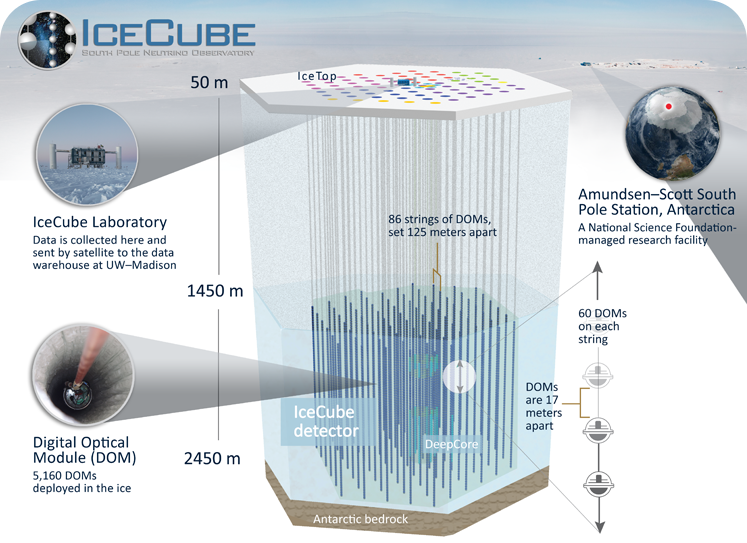
\includegraphics[width=\textwidth]{chapter5/img/icecube_detector_sm.png}
\caption{Illustration of the IceCube South Pole neutrino observatory.}
\label{fig:ICgeometry}
\end{figure} 

\begin{figure}
\centering
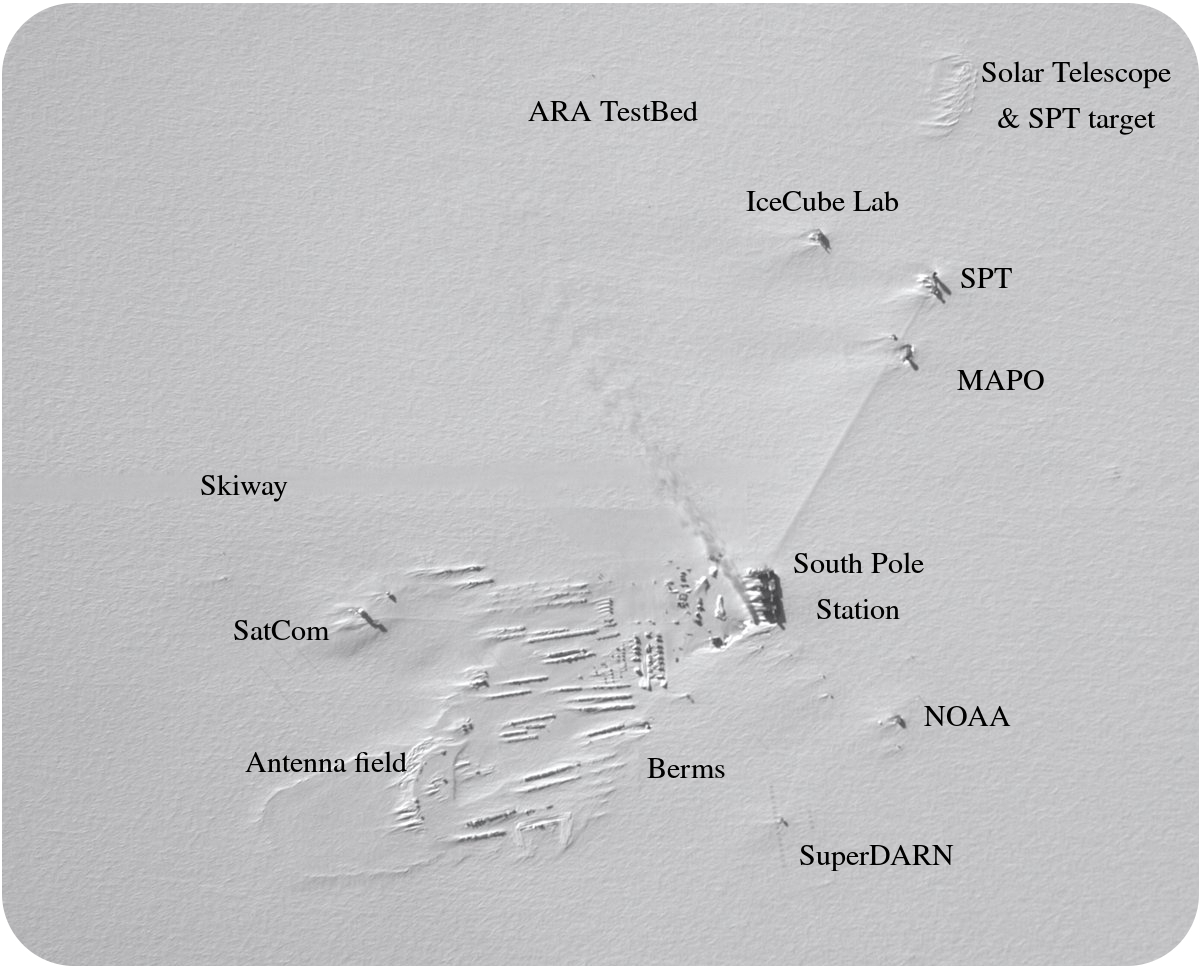
\includegraphics[width=0.75\textwidth]{chapter5/img/SouthPole_3.jpg}
\caption{Aerial view of the South Pole. The main buildings and experimental setups are indicated in the figure. The exhaust of the South Pole Station is also visible.}
\label{fig:aerialview}
\end{figure} 

\section{Geometry}
The IceCube detector consists of three main parts that act as different purpose physics detectors. 
The \textit{in-ice IceCube} detector is the main component and consists of 4680 digital optical modules. In its core, a denser subdetector, \textit{DeepCore}, significantly enhances the capabilities for low-energy events of the observatory in a limited volume. The center of the DeepCore array consists of 480 sensors.
On the surface of the ice, water tanks with optical modules inside are spread out over an area of approximately 1 km$^2$ and make up the \textit{IceTop detector}. This surface array was built as a cosmic ray detector and veto for the in-ice array.  The three components combined make the facility a multipurpose physics detector. Figure \ref{fig:ICgeometry} shows the layout of the detector.

\subsection{In-ice array}
The in-ice array consists of 4680 digital optical modules (DOMs) that are able to register light that is scattered and propagated through the ice (more info about these modules can be found in Section \ref{subsec:doms}). The DOMs are attached to cables and are frozen in the ice. In total, 78 of these ``strings'' were frozen into boreholes and spread out over a cubic kilometer in a hexagonal shape. Because only the deep ice is transparent, the DOMs are attached to the strings starting from a depth of 1450 meters to 2450 meters. The strings, as viewed from above, are spaced about 125 meters apart and along each string, 60 DOMs are attached with a vertical separation of 17 meters. This design was chosen in order to meet up to the primary science requirement of detecting astrophysical neutrinos in the energy range of $\mathcal{O}$(TeV)– $\mathcal{O}$(PeV).

 
\subsection{DeepCore}
\label{subsec:DC}
A subset of in-ice DOMs is deployed along eight extra strings in the central region of the in-ice array. The optical modules are deployed deeper than 1750 meter with a denser instrumented volume. Seven additional strings, belonging to the standard in-ice strings, are also combined with the DeepCore strings to optimize the instrumented volume for this detector. The inter-string spacing on the eight specialized DeepCore strings varies from 41 meters to 105 meters. The DOM-to-DOM spacing is 7 meters for the bottom 50 optical modules (which are deployed at depths of 2100 to 2450 meters). The remaining 10 DOMs on each string are located at depths above 2000 meters deep with a spacing of 10 meters. This extra ``layer'' surves as a veto for downgoing atmospheric muons. Each string is instrumented with 60 DOMs, resulting in a total of 480 DOMs. Instrumentation in the ice between 2000 to 2100 meters proved to be less useful due to the \textit{dust layer} (see Section \ref{sec:ice}) and was therefore left out. Six out of the eight specialized strings are also instrumented with DOMs using PMTs of higher quantum efficiency. The two remaining strings are instrumented with regular IceCube DOMs. A layout of the in-ice array is given in Figure \ref{fig:layoutIC}.

The DeepCore design allows us to detect neutrinos of much lower energies in the range of $\mathcal{O}$(10 GeV)– $\mathcal{O}$(100 GeV). Experiments for neutrino oscillation experiments, WIMP dark matter annihilation, galactic supernova neutrinos and point sources are made possible, or more feasible, with this dense subarray \cite{Collaboration:2011ym}.

\begin{figure}[t]
\centering
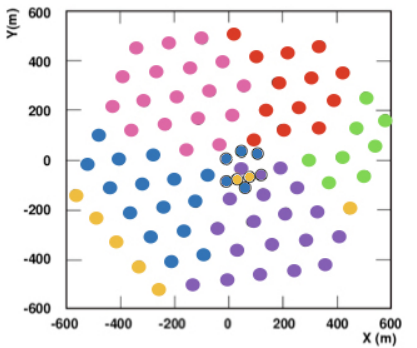
\includegraphics[width=0.5\textwidth]{chapter5/img/layoutIC.png}
\caption{Layout of the IceCube (regular) and DeepCore strings (black edge). The string color scheme represents different deployment seasons (04-05: orange, 05-06: green, 06-07: red, 07-08: pink, 08-09: purple, 09-10: blue, 10-11: yellow). Figure from Ref. \cite{Choma:2018zbe}, with minor corrections.}
\label{fig:layoutIC}
\end{figure}

\subsection{IceTop}
IceTop is a cosmic ray air shower array, located on the surface of the ice and 2835 meters above sea level. As discussed in Chapter \ref{ch:cr}, air showers die out when they are propagating to Earth's surface but as a consequence of the high altitude of IceTop, showers are observed near maximum\footnote{The height of the shower where the maximum number of particles are produced in an air shower is often referred to as the ``shower maximum''.}, resulting in a good energy resolution for the detector. This is important if one wants to measure changes in composition as a function of energy. In total, 162 ice-filled tanks are distributed in 81 stations (two tanks per station) in a grid similar to the in-ice array. Like the denser DeepCore infill, there are eight stations in the center of IceTop placed more closely together. 

The two tanks per station are separated 10 meters apart from each other and each tank contains two IceCube DOMs. One is operated at a ``low-gain'' and one at ``high-gain'', making them more suitable for air shower detection. The tanks measure the Cherenkov light that is produced in the ice of a tank due to the particles in a shower (electrons, positrons, muons and hadrons). The IceTop design allows to fully cover the knee of the energy spectrum and is primarily sensitive from PeV to EeV energies. The denser infill allows the threshold to be lowered to 100 TeV. The detector is used in studies of the composition, high-$p_T$ muons, etc. 

\subsection{IceCube coordinate system}
When referring to positions and directions, one has to define a coordinate system that is be able to uniquely define these variables. The system used in the IceCube collaboration is shown in Figure \ref{fig:coordinates}.\\

\begin{figure}[t]
\centering
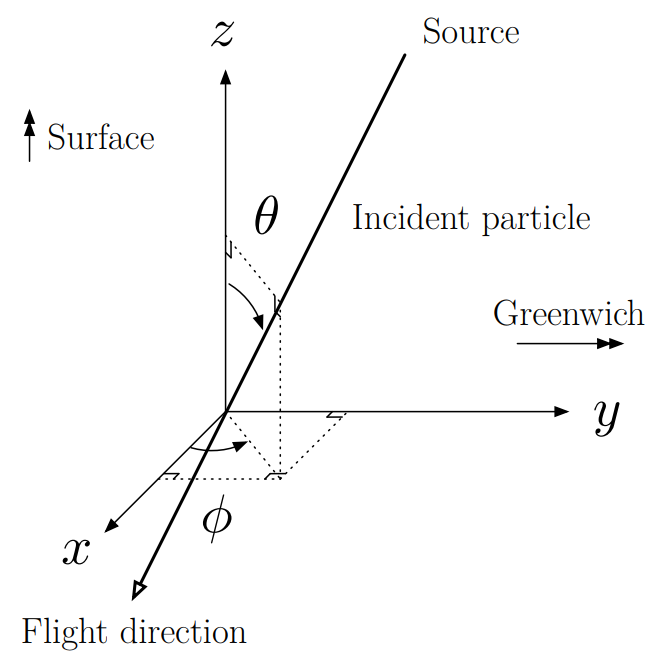
\includegraphics[width=0.5\textwidth]{chapter7/img/CoordinateSystem.png}
\caption{The IceCube coordinate system.}
\label{fig:coordinates}
\end{figure}

\noindent The center of the coordinate system is set close to the geometric center of the detector, at about 2000 m below the surface of the ice. The y-axis of the coordinate system is aligned with the Prime Meridian pointing toward Greenwich (United Kingdom). The x-axis is set perpendicular to the y-axis pointing in a, 90$^\circ$ clockwise direction. The z-axis is set perpendicular to the xy-plane, pointing upwards, normal to the Earth's surface.

A particle's direction is defined with zenith and azimuth angles, $\theta$ and $\phi$ respectively. The zenith angle is measured relative to the positive z-axis and the azimuth angle is measured counterclockwise from the positive xy-plane.



\section{Hardware components}
\subsection{Digital optical modules}
\label{subsec:doms}
The Digital Optical Modules, or DOMs, convert light into electrical signals and have the necessary hardware installed to perform some basic processing of the electrical pulses. A downward facing 10''-diameter photomultiplier tube (PMT) is set with a high voltage of 2 kV, resulting in a gain of $10^7$ \cite{Aartsen:2016nxy}. The amplitude of the resulting waveforms ranges from 1 mV up to and beyond the linearity limit of the PMT ($\sim2$ V) with the width ranging from 12 ns to 1500 ns. This wide dynamic range of the waveform is processed by onboard electronics: the main board and delay board. The main board controls all the devices in the DOM (high voltage power supply for the PMT, the flasher board and pressure, temperature, and power supply voltage monitor sensors), digitizes the PMT waveforms, communicates with the data acquisition (DAQ) on the surface, houses an internal clock that is regularly calibrated with the DAQ on the surface and exchanges pulses with the adjacent DOMs.
An illustration of the mechanical components of the optical module and a schematic view of the data flow starting from the PMT is shown in Figure \ref{fig:DOM}. The optical module is housed in a 13''-glass sphere of 0.5'' thick made from borosilicate. It is separated into two halves and held together with an aluminium waistband. The sphere was tested up to 690 bar hydrostatic pressure and is able to withstand the enormous pressure that the DOM is exposed to deep within the ice and during freezing (see Section \ref{sec:deployment}). A penetrator inside the glass sphere brings out three wires pairs housed in a cable. One wire pair is connected to the string and ultimately to the IceCube Laboratory (see Section \ref{subsec:icl}), the other two wires to the neighboring DOMs directly above and below for local coincidence pulses (see Section \ref{subsec:cablesystems}). A detailed description is given in the detector paper \cite{Aartsen:2016nxy}.

\begin{figure}
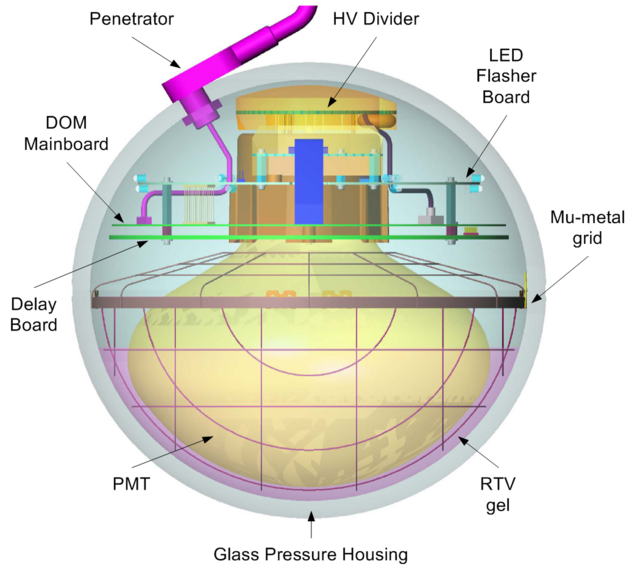
\includegraphics[width=0.48\textwidth]{chapter5/img/DOM-Picture.png}
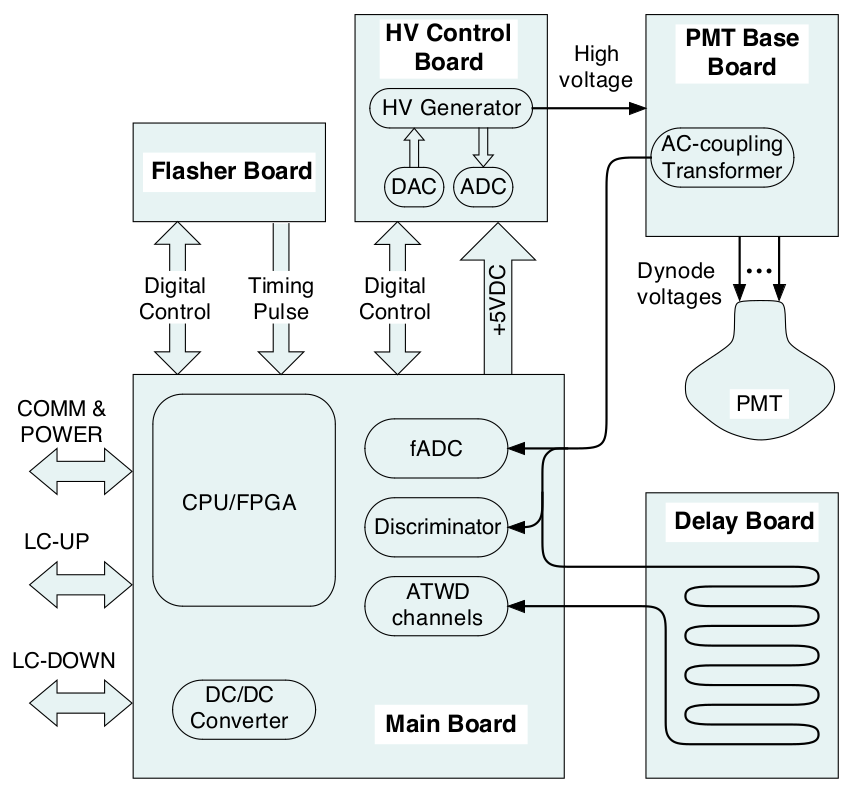
\includegraphics[width=0.48\textwidth]{chapter5/img/electronicsDOM.png}
\caption{\textit{Left:} illustration of the mechanical DOM components. \textit{Right}: Scheme of the functional connections.}
\label{fig:DOM}
\end{figure}

\subsubsection{PMTs}
The 10'' (or 25 cm) diameter PMT comes in two types: Hamamatsu R7081-02 for standard IceCube DOMs and a high-quantum-efficiency (HQE) version, Hamamatsu R7081-02MOD for the specialized DeepCore strings \cite{Abbasi:2010vc}. The peak quantum efficiency is around 25\% (34\% for HQE) at a wavelength of approximately 390 nm. However, the total acceptance of the optical module is the convolution of the quantum efficiency with the glass transmission (93\% at 400 nm, decreasing to 50\% at 340 nm and 10\% at 315 nm at a normal incidence). The resulting acceptance is illustrated in Figure \ref{fig:acceptance}. The PMTs face downwards and are housed in a mu-metal grid to shield them from the Earth magnetic field and a silicone gel necessary for optical coupling and mechanical support.

\begin{figure}[ht]
\centering
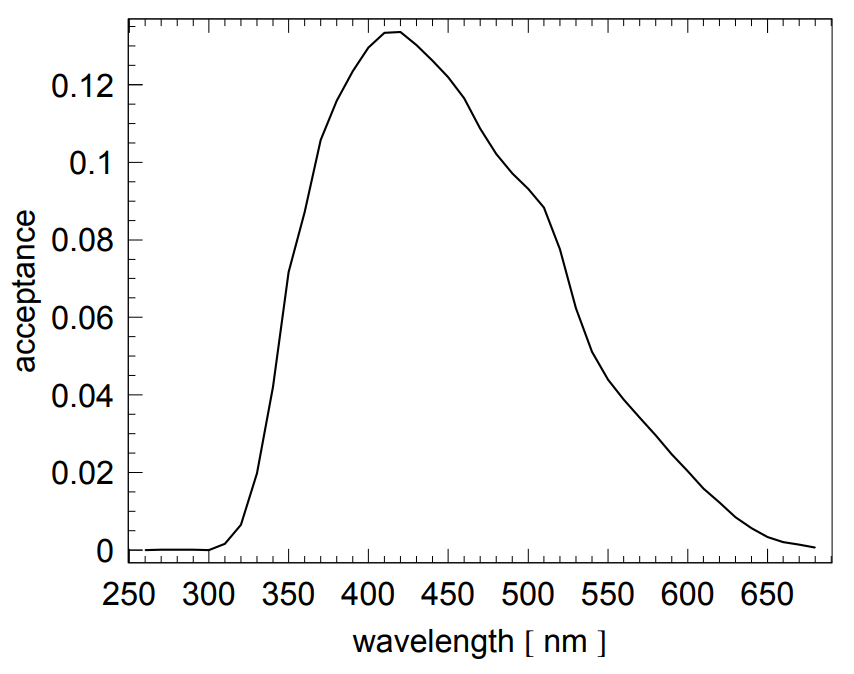
\includegraphics[width=0.7\textwidth]{chapter5/img/acceptanceDOM.png}
\caption{Fraction of photons arriving from a direction parallel to the PMT axis in function of the photon wavelength. Glass and gel transmission, PMT quantum and collection efficiencies are all included. Figure from Ref. \cite{Aartsen:2013rt}.}
\label{fig:acceptance}
\end{figure}


\subsubsection{Main board and delay board}
\label{subsec:mainboard}
The PMT signals are sent to two ATWD (Analog Transient Waveform Digitizer) and one fast ADC (fADC) with a delay of about 75 ns. This delay is necessary because signals are only processed if the signal exceeds a voltage that corresponds to 0.25 PE (one PE is the voltage that typically corresponds to the voltage produced by a single photoelectron). Once this threshold is crossed, the signal is compressed and included in a ``DOMlaunch'' or ``hit''. Signals that pass the local coincidence requirement (see Section \ref{subsec:cablesystems}) have their full waveforms compressed, whereas for isolated events only a time stamp and brief charge summary is sent. For each hit, an FPGA  (Field Programmable Gate Array) opens up one of the two ATWD chips. Each of the two chips is provided with three amplifier gains with nominal values of 16, 2 and 0.25. Most pulses use the highest-gain channel while the other lower-gain recordings are used as needed when pulses reach 75\% of the range of a higher-gain channel. The ATWD recording duration is 427 ns, which should include light that is produced within tens of meters of a DOM. The slower fADC is used when light reaches the DOM after the ATWD time window and samples continuously. The FPGA is programmed to save an interval of 6.4 $\mu$s after the launch. ATWD chips sample the input voltage at 300 Msps, followed by a 10-bit digitization. The fADC captures the information with a 10-bit 40 Msps.

The two sets of ATWD chips are operated alternately in order to reduce deadtime. After 50 ns, the second chip is available to be launched during the digitization step of the first. The digitization procedure is terminated for isolated hits and the ATWD is reset, reducing the DOM dead time.\\

\noindent The delay board consists of a 10 m-long copper trace that delays the signal for 75 ns, necessary to be able to record the full waveform before the discriminator threshold of 0.25 PE is exceeded.

\subsubsection{Flasher board}
\label{subsub:flasher}
To be able to characterize the ice and simulate light propagation, each DOM was instrumented with 12 LEDs that are aimed in six different azimuth angles (with 60$^\circ$ spacing) and along two different zenith angles. The LEDs were chosen to have a wavelength spectrum centered at around 400 nm to approximate the typical wavelength of detected Cherenkov photons. Flasher data is used for:
\vspace{2mm}
\begin{itemize}
\item verifying the timing response of the DOMs throughout the analysis software chain;
\item measuring the position of the deployed DOMs in ice;
\item measuring the optical properties of the ice (see Section \ref{sec:ice});
\item verifying the performance of shower reconstruction algorithms in measuring position, direction and energy.
\end{itemize}



\subsection{Calibration}
\label{subsec:calibration}
Regular calibration of the components is necessary to be able to convert the DOM waveforms to reliable and comparable physical units. Optical efficiencies of the optical modules were determined in the lab before deployment and are also done \textit{in situ} with calibration procedures.

Some of these procedures do not allow for simultaneous data-taking and are performed as little as possible, without losing significant confidence in the calibration of the devices. For example, in-ice DOMs are calibrated yearly with the DOMCal procedure, whereas global time calibration can be done in parallel with data-taking and is provided by the RAPCal procedure.

As they result in the vast majority of the background hits, \textit{dark noise} needs to be properly understood for low-energy neutrino analyses, supernova searches, and detector simulations. The total rate of dark noise averages at around 560 Hz for in-ice DOMs and 780 Hz for HQE DOMs. The origins of the noise are non-trivial and include electronic noise, thermionic emission, Cherenkov light from radioactive decays, field emission within the PMT, and scintillation/luminescence in the glass of the PMT and pressure sphere. They are simulated with a combination of uncorrelated (Poissonian) noise and a correlated component. The temperature dependence of the noise rate was determined by combining a measured temperature profile of the South Pole ice cap with a fit of the Poissonian expectation of the total dark noise rate to every individual DOM, and was verified in lab measurements. The seasonal variations of the dark noise rates are below 1\%, but are tracked over time and updated yearly in a database.\\

\noindent More information about these and other calibration procedures can be found in Ref. \cite{Aartsen:2016nxy}.

\subsection{Cable systems}
\label{subsec:cablesystems}
\begin{figure}
\centering
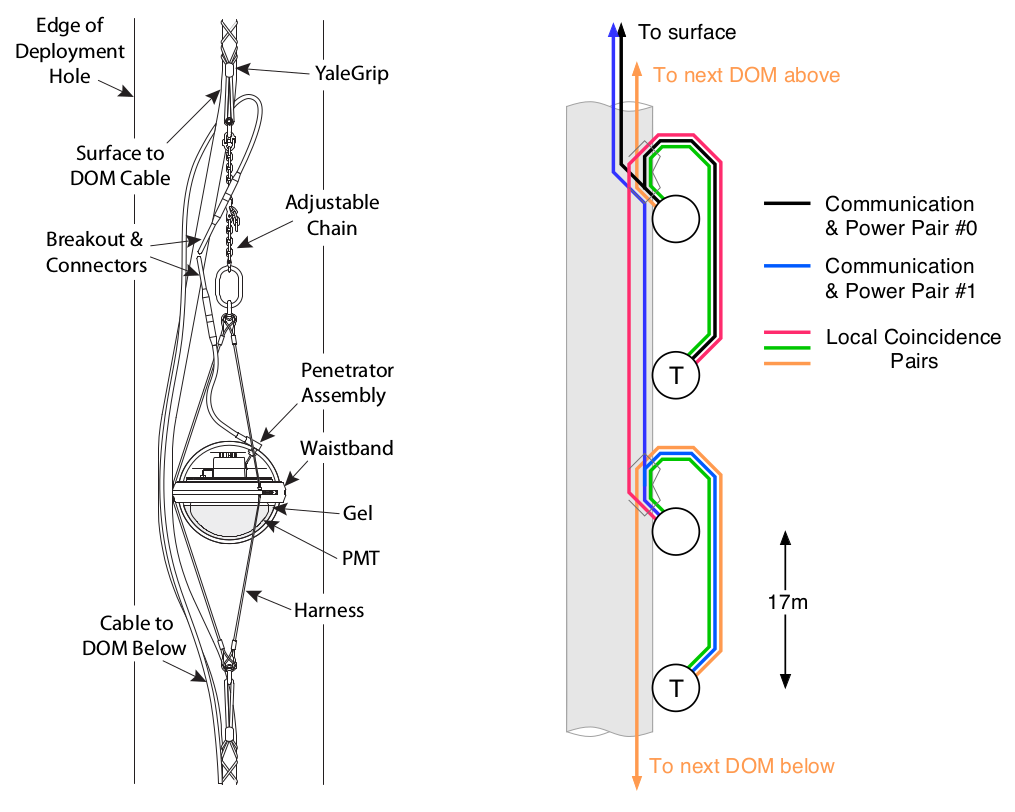
\includegraphics[width=0.9\textwidth]{chapter5/img/cablelayout.png}
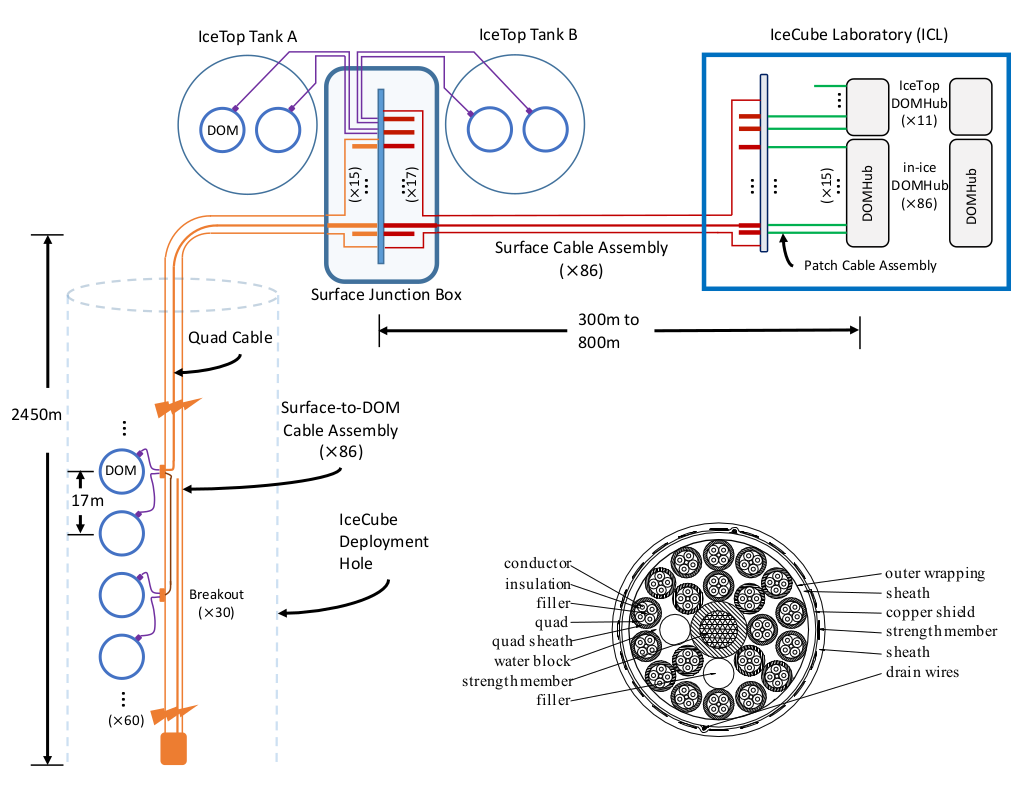
\includegraphics[width=0.9\textwidth]{chapter5/img/cableSchematic_withcable.png}
\caption{\textit{Top}: Sketch of DOM cabling and schematic overview. The modules are connected to their nearest neighbors and the string. \textit{Bottom}: General schematic overview of the IceCube cabling system and the connection between all components together with an in-ice cable cross section. Illustrations from Ref. \cite{Aartsen:2016nxy}.}
\label{fig:cable}
\end{figure}

The DOMs are the eyes of the detector, but the cable system connects all the modules together and links them to the readout hardware at the surface. The in-ice cables, 2505 m long, are each connected to 60 DOMs and terminate at a Surface Junction Box (SJB) between IceTop tanks. IceTop tanks also connect to the SJB. A surface cable was trenched 1 m deep at the time of deployment and runs to the IceCube Laboratory. One cable consists of 20 ``quads'', a construction of four twisted wires. Four quads provide special instrumentation and local coincidence between connections and one is a spare. The remaining 15 quads are each connected to four DOMs with two wire pairs. A wire pair connects two adjacent DOMs and is attached to connectors at 30 breakouts spaced 34 m apart as can be seen in Figure \ref{fig:cable}. Each DOM is connected to three wire pairs. One wire pair is used for bi-directional communication to the surface and power. The two remaining wires are dedicated to determince \textit{Local Coincidence (LC)}. Each DOM is connected to its nearest neighbor above and below. If nearest or next-to-nearest neighbors are hit within a time window of $\pm$ 1 $\mu$s, the hits are said to be in Hard Local Coincidence (HLC). Isolated hits are referred to as Soft Local Coincidence (SLC). Most DOM hits originate from dark noise (see Section \ref{subsec:calibration}) and are not in HLC. Light originating from particles traveling through matter is more likely to trigger DOMs in close proximity. Therefore, LC requirements are able to drastically reduce the noise rate.

\subsection{IceCube laboratory}
\label{subsec:icl}
The central building to which the modules of all the detectors are connected is the IceCube Laboratory (ICL). Cables/strings from the arrays run up two cable towers on either sides of the structure. A picture of the ICL is shown as the header image of this chapter (pg. \pageref{ch:icecube}); one of the towers is visible. Inside the main part of the building is a server room to which the cables in the towers are connected. All data acquisition and online filtering computers are housed inside the server room together with the main IceCube computing system called the ``South Pole System'' (more information on this in Section \ref{sec:datataking}).


\section{Deployment}
\label{sec:deployment}
In total, 86 holes had to be drilled for all IceCube and DeepCore strings. The surface consists of a 50 m snow and firn region with a gradual transition to ice. The ice was melted with a 5 MW Enhanced Hot Water Drill (EHWD) capable of drilling about 1 hole per 48 hours. The holes were 60 cm in diameter, providing enough clearance for the optical modules that were 35 cm in diameter, and with contingency time for delays that meant holes could shrink due to refreezing. Because melting snow and firn with hot water is not practical, a specialized drill with copper tubing through which hot water flows was used to melt the firn by contact.

The IceCube drilling was completed in seven field seasons during Antarctic summers (early November to mid-January). The first season started in 2004-2005 and construction ended in 2010-2011. 
%At the end of each season, the Seasonal Equipment Site (SES) that provided electricity and a stable supply of hot pressurized water had to be decomissioned and positioned at the site for the next drilling season due to its size and complexity. From the SES a more flexible Tower Operations Site (TOS) was linked and held the drill tower, operations building, and hose and cable reels. There were two towers, where one was set up for drilling while the second one was still being used for deployment of the cables.

After drilling one hole, all 60 DOMs were lowered one by one and connected to each other with the penetrator assembly as shown in Figure \ref{fig:cable}. After deployment of all DOMs, the remaining 1,\.5 km of in-ice cable was lowered into the hole (known as the ``drop phase''). The top of the cable was then secured by an anchor trenched in the snow and connected to the Surface Junction Box. 

In total, 5484 (5160 IC + 324 IT) optical modules were deployed and as of 2018, there are 5396 still in data-taking mode (98.4\%). There were 55 DOMs that failed almost immediatly during freeze-in, while 34 DOM failures occurred after deployment. This number includes modules on a wire pair that are taken out when the partner DOM on the same pair failed. The mean failure rate is estimated to be around $(4.1 \pm 1.2)$ yr$^{-1}$, which results in a survival fraction of $(97.4 \pm 0.3)\%$ in 2030.

\section{Data taking}
\label{sec:datataking}

\begin{figure}[ht]
\centering
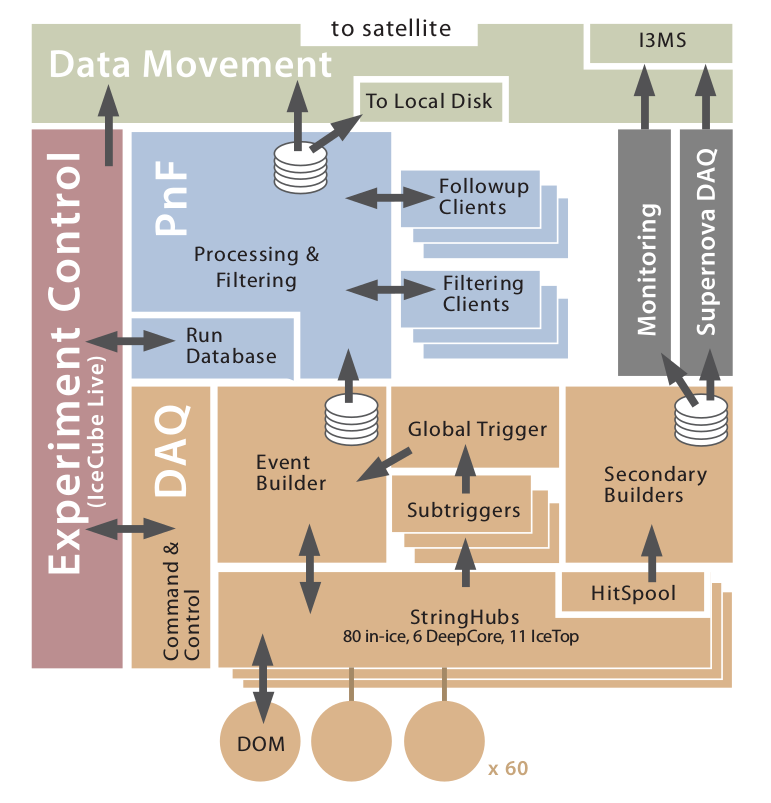
\includegraphics[width=0.7\textwidth]{chapter5/img/dataflow.png}
\caption{Schematic overview of the data flow in the primary IceCube online systems.}
\label{fig:dataflow}
\end{figure}
First processing of the photon detection is done inside the DOM. After digitization, the waveforms are sent along the cable/string to which all DOMs are attached and that runs to the ICL. Each one of the strings is connected to one of the DOMHubs, which together with servers that run various online systems, comprises the South Pole System (SPS). An overview is given in Figure \ref{fig:dataflow}.

The data acquisition (DAQ) system is run on the DOMHubs and recognizes patterns in hits that are most likely caused by particle interactions with the use of the implemented triggers and filters (see below). This combination of hits is called an ``event''. Most of the DAQ data rate originates from atmospheric muons with an event rate averaging 2.7 kHz. The total bandwith saved to tape/disk (see Section \ref{subsec:datahandling}) is approximately 1 TB/day.

To implement possible changes in the detector settings, triggers, or filters, a full physics run spans over one year, starting in May and ending in May the following year. Data is recorded in smaller 8 hour runs, where each run has a unique run number. Over the years, with the use of both online and on-site automatic alerts, the total uptime of the detector has a steady increase of clean uptime (usable data) from 89.75\% in 2011 to 98.89\% in 2018.

\subsection{Triggers}
\label{subsec:triggers}
Aside from the discriminator thresholds in the module (see Section \ref{subsec:mainboard}), a system of triggers is set up to further reduce the noise rate and refine searches for physics events. Below, a short description of the triggers is given. An overview of the trigger settings is given in Table \ref{tab:trigger}. 

\vspace{2mm}
\begin{itemize}
\item The most important trigger is the Simple Multiplicity Trigger (SMT) used for the IceCube, DeepCore and IceTop arrays. The trigger setting requires a certain number of hits within a time window of the order of a couple of $\mu$s without any locality requirements.
\item The Volume Trigger requires less HLC hits, but they have to be clustered in a certain cylindrical volume. 
\item Locality conditions are powerful for low-energy events that do not reach far in the detector but are more prone to produce hits in a small volume and time window. Therefore, a dedicated String Trigger was designed for low-energetic upgoing events passing along a single string. 
\item IceCube is also sensitive to hypothetical massive particles moving at subrelativistic speeds: magnetic monopoles. Therefore, a dedicated Slow Particle (SLOP) trigger has been developed. It searches for triplets of HLC pairs within a window, $T_{\textrm{max}}$, and removes HLC pairs within a time window, $T_{\textrm{prox}}$, to remove hits originating from particles traveling at the speed of light. Other velocity and geometric requirements are set with the inner angle between triplets, $\alpha_{\textrm{min}}$ and the ``velocity'' along the sides of the triangle.
\item A Fixed Rate Trigger (FRT) reads out hit data from the full detector at fixed intervals, useful for DOM noise studies.
\end{itemize}
\vspace{2mm}

\noindent If a trigger condition is fulfilled, the start of the trigger window is determined as the first HLC hit of the active volume of the trigger. The minimum length of the triggered window slides along with the hits until there is no more HLC after the last hit within the set minimum time window. The length of a triggered set of hits can therefore be longer than the minimum trigger window. As one event is able to fulfill multiple trigger requirements, the (sub)triggers are merged into one Global Trigger while keeping the information on the individual triggers. This data is subsequently sent to the Event Builder that writes DAQ events (also called \textit{Q frames}) to a temporary file that is saved when it reaches a certain size. These events are eventually re-split into physics events (\textit{P frames}) corresponding to a certain subtrigger before reconstruction and analysis. An example of a Global Trigger, here mostly determined by the very long SLOP trigger, is shown in Figure \ref{fig:globaltrigger}.

All triggers read out all SLC/HLC hits of all DOMs, even the ones not directly involved in the trigger construction. For this, they use the StringHub software component located on every DOMHub that is able of caching SLC and HLC hits in memory. Hits before and after the trigger window are also saved to the event to add information of early and late pulses. This is typically 4 $\mu$s before and 6 $\mu$s after the trigger window for in-ice triggers. 



%The StringHub is also able to save local ``HitSpool'' on-disc data and later request it if necessary from the Event Builder. This HitSpool data is able to store up to 16 hours of all waveforms overwriting the oldest data first and originally intended for the detection of Galactic supernovae. Such an event would give rise to a steady increase in apparent dark noise from its low-energy neutrinos without fulfilling the standard trigger requirements. Over the years, the HitSpool data has found multiple other usecases such as a neutron echo analysis, searching for delayed neutrons from hadronic interactions \cite{Aartsen:2017mnf}. 

\begin{figure}[t]
\centering
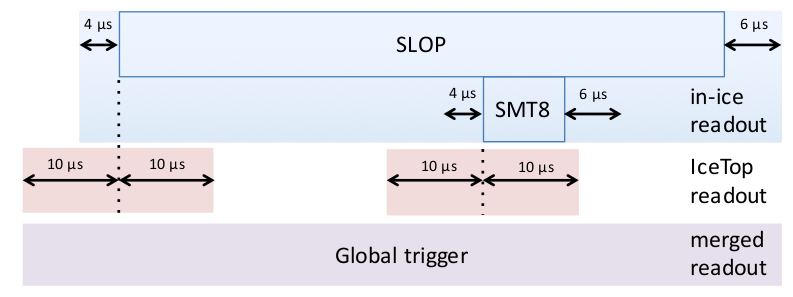
\includegraphics[width=0.8\textwidth]{chapter5/img/globaltrigger.png}
\caption{Example of a global trigger construction. Multiple triggers are combined due to their overlap with the long SLOP trigger.}
\label{fig:globaltrigger}
\end{figure}


\begin{table}[]
\centering
\caption{Parameter settings of triggers (as of May 2016) and typical trigger rates.}
\label{tab:trigger}
\resizebox{\textwidth}{!}{%
\begin{tabular}{|l|r|r|r|c|c|r|r|}
\hline
\cellcolor[HTML]{F1A91E} & \multicolumn{1}{c|}{\cellcolor[HTML]{F1A91E}} & \multicolumn{1}{c|}{\cellcolor[HTML]{F1A91E}} & \multicolumn{1}{c|}{\cellcolor[HTML]{F1A91E}} & \multicolumn{2}{c|}{\cellcolor[HTML]{F1A91E}Readout Window ($\mu$s)} & \multicolumn{1}{c|}{\cellcolor[HTML]{F1A91E}} & \multicolumn{1}{c|}{\cellcolor[HTML]{F1A91E}} \\ \cline{5-6}
\multirow{-2}{*}{\cellcolor[HTML]{F1A91E}Trigger} & \multicolumn{1}{c|}{\multirow{-2}{*}{\cellcolor[HTML]{F1A91E}DOM set}} & \multicolumn{1}{c|}{\multirow{-2}{*}{\cellcolor[HTML]{F1A91E}$N$ HLC hits}} & \multicolumn{1}{c|}{\multirow{-2}{*}{\cellcolor[HTML]{F1A91E}Trigger Window ($\mu$s)}} & \multicolumn{1}{c|}{\cellcolor[HTML]{F1A91E}\ \ \ \ IC\ \ \ \ } & \multicolumn{1}{c|}{\cellcolor[HTML]{F1A91E}\ \ \ \ IT \ \ \ \ } & \multicolumn{1}{c|}{\multirow{-2}{*}{\cellcolor[HTML]{F1A91E}Topology}} & \multicolumn{1}{c|}{\multirow{-2}{*}{\cellcolor[HTML]{F1A91E}Rate (Hz)}} \\ \hline
\textbf{SMT} & \textbf{in-ice} & 8 & 5 & $-4,+6$ & $\pm10$ & - & 2100 \\ \hline
\textbf{SMT} & \textbf{DeepCore} & 3 & 2.5 & $-4,+6$ & $\pm10$ & - & 250 \\ \hline
SMT & IceTop & 6 & 5 & $\pm10$ & $\pm10$ & - & 25 \\ \hline
\textbf{Volume} & \textbf{in-ice} & 4 & 1 & $-4,+6$ & $\pm10$ & cylinder (r = 175 m, h = 75 m) & 3700 \\ \hline
Volume & IceTop & 4 & 0.2 & $\pm10$ & $\pm10$ & cylinder (r = 60 m, h = 10 m) & 4 \\ \hline
\textbf{String} & \textbf{in-ice} & 5 & 1.5 & $-4,+6$ & $\pm10$ & 7 adjacent vertical DOMs & 2200 \\ \hline
 &  &  & $T_{\textrm{prox}} = 2.5$ &  &  &  &  \\ \cline{4-4}
 &  &  & $T_{\textrm{min}} = 0$ &  &  &  &  \\ \cline{4-4}
\multirow{-3}{*}{SLOP} & \multirow{-3}{*}{in-ice} & \multirow{-3}{*}{$N_{\textrm{triplet}}$} & $T_{\textrm{max}} = 500$ & \multirow{-3}{*}{$-4,+6$} & \multirow{-3}{*}{$\pm10$} & \multirow{-3}{*}{$\alpha_{\textrm{min}} = 140^\circ, v^{\textrm{max}}_{\textrm{rel}} = 0.5$} & \multirow{-3}{*}{12} \\ \hline
FRT & all & - & - &  \multicolumn{2}{c|}{Combined: 10000} & - & 0.003 \\ \hline
\end{tabular}%
}
\end{table}



\subsection{Filters}
\label{subsec:filters}
Events are sent through the online Processing and Filtering (PnF) system for additional processing. First, the triggered events have their waveforms further compressed using the Super Data Storage and Transfer format (SuperDST), which uses only 9\% of the storage size of the full waveform information. Very fast, basic reconstructions are run on the SuperDST waveforms to compute the vertex position, energy, direction and goodness-of-fit that are necessary for the filter selections of possible interesting events.

Around 25 filters search for a wide range of different types of particle interactions, ranging from low-energy neutrinos for oscillation measurements to the highest-energy neutrino interactions illuminating large parts of the detector. Some filters are designed to look for neutrino events of wide astrophysical interest to the scientific community and trigger allerts that are distributed to followup observatories worldwide. One example is the ``EHE alert'' that searches for Extremely High Energy neutrinos that are most likely of astrophysical origin \cite{Aartsen:2016lmt}. Another example is the Gamma Follow Up alert that notifies the MAGIC and VERITAS collaborations when significant bursts of neutrinos from known high-energy gamma-ray sources over periods up to 3 weeks occur \cite{1412973}. Other filters look for events that could be caused by muons, WIMPs, monopoles, etc. The filters that were used in this analysis are given in Section \ref{sec:filterselection}.

As a bonus, filtering reduces the data volume to a level of around 90 Gb/day, which is small enough to transfer to the North using a satellite.

\subsection{Data handling}
\label{subsec:datahandling}
Most of the data is processed with the PnF system. The geometry, calibration, and detector status (GCD) information from each 8 hour run is sent via the same satellite transfer that is used for the continuously running PnF system. All the raw waveforms were written to tape before that system was retired in 2015. Since then, disks have been used to store the remaining archival data. This raw data is shipped to the North every year and is used if reprocessing of data is necessary. An example is the SPE correction for all runs starting from 2010 to 2016 referred to as \textit{pass2 data} \cite{pass2}. \\

\noindent Files are stored in IceCube specific files and are called \textit{i3files} \index{i3file}.

\section{Antarctic ice}
\label{sec:ice}
The ice, in which the optical modules are frozen, acts as the propagation medium for the light that is produced by relativistic particles. Therefore, the parameterization of the ice is of great importance for good reconstructions and reliable simulations. The relativistic particles that travel through the ice produce photons in a Cherenkov cone of around 41$^\circ$ (see Section \ref{sec:cherenkoveffect}). How these photons further propagate from the point of emission to the receiving sensors is determined by the absorption and scattering within the ice. The most important parameters necessary to describe the photon propagation in ice are:
\vspace{2mm}
\begin{itemize}
\item the average distance to absorption,
\item the average distance between successive scatters of photons, and 
\item the angular distribution of the new direction of a photon at each given scattering point.
\end{itemize}
\vspace{2mm}
There has been a large effort into measuring and modeling the Antarctic ice that is still ongoing. A good summary (although is a bit outdated as it does not include ice anisotropy effects, cable shadowing and DOM tilts) can be found in Ref. \cite{Aartsen:2013rt}.

\subsection{Ice simulation}
\label{subsec:icesimulation}
The ice is modeled by the six-parameter ice model introduced in Ref. \cite{Ackermann:2006pva}. Flasher data from LEDs is used to fit the model to data (see Section  \ref{subsub:flasher}). In this model, the ice is described by a table of depth-dependent parameters $b_e(400)$ and $a_{dust}(400)$ related to scattering and absorption at a wavelength of 400 nm. These two parameters depend on the relative temperature $\delta \tau$, which changes in function of depth, and six global parameters. The effective scattering coefficient is equal to $b_e = b \cdot \left( 1-\langle \cos \theta \rangle \right)$, where $b$ is the geometrical scattering coefficient that determines the average distance between successive scatters and $\theta$ is the deflection angle at each scatter. The absorption coefficient $a$ determines the average distance traveled by a photon before it is absorbed and is the sum of two components: one due to dust and the other a temperature dependent component for pure ice.

\begin{equation}
b_e(\lambda)  = b_e(400) \cdot \left( \frac{\lambda}{400}\right)^{-\alpha},
\end{equation}

\begin{equation}
\begin{split}
a(\lambda) &= a_{dust}(\lambda) + A e^{-B/\lambda} \cdot (1+0.01 \cdot \delta \tau), \\
&\textrm{with} \ \ \ a_{dust}(\lambda) = a_{dust}(400) \cdot \left( \frac{\lambda}{400}\right)^{-\kappa}.
\end{split}
\end{equation}
$\alpha, \kappa, A \textrm{ and } B$ are determined in Ref. \cite{Ackermann:2006pva}\footnote{The remaining two parameters $D$ and $E$ were not used here.}, $\delta \tau$ is equal to

\begin{equation}
\begin{split}
&\delta \tau(d) = T(d) - T(1730 \textrm{m}), \\ 
\textrm{with} \ \ T(d) = 221.5 &- 0.00045319 \cdot d + 5.822 \cdot 10^{-6} \cdot d^2,
\end{split}
\end{equation}
where $d$ is the relative depth compared to the center of AMANDA (1730 m depth). Using flasher data with 400 nm wavelengths, it is possible to measure the values of $b_e(400)$ and $a_{dust}(400)$ at certain depths and use the six-parameter ice model to extrapolate scattering and absorption for other wavelengths. 

In 2008, a flasher run was launched where each DOM on string 63 was producing flashes. The layout of the detector at the time of the flasher run and results of fits to $b_{e}(400)$ and $a(400)$ vs. depth can be found in Figure \ref{fig:2008config}. At a depth between 2000 meters and 2100 meters, a large increase in scattering and absorption is clearly visible. A \textit{dust layer}, presumably originating from volcanic ash, is characterized by an increase of dust in the ice, responsible for the higher scattering and absorption factors.

\begin{figure}[t]
\begin{minipage}{6in}
  \centering
  \raisebox{-0.5\height}{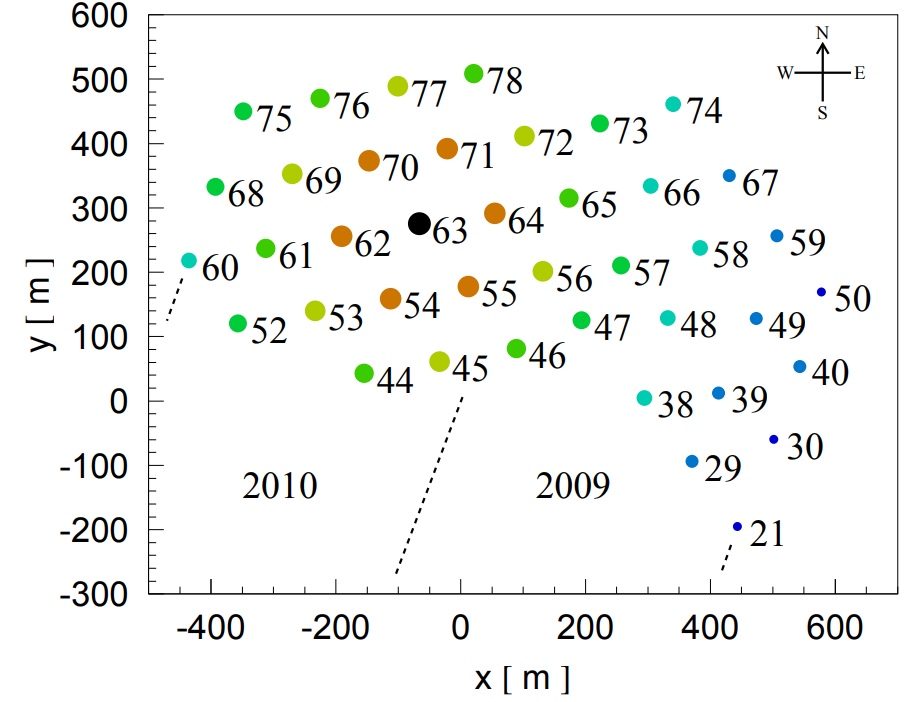
\includegraphics[height=2in]{chapter5/img/2008config.png}}
  \hspace*{.7in}
  \raisebox{-0.5\height}{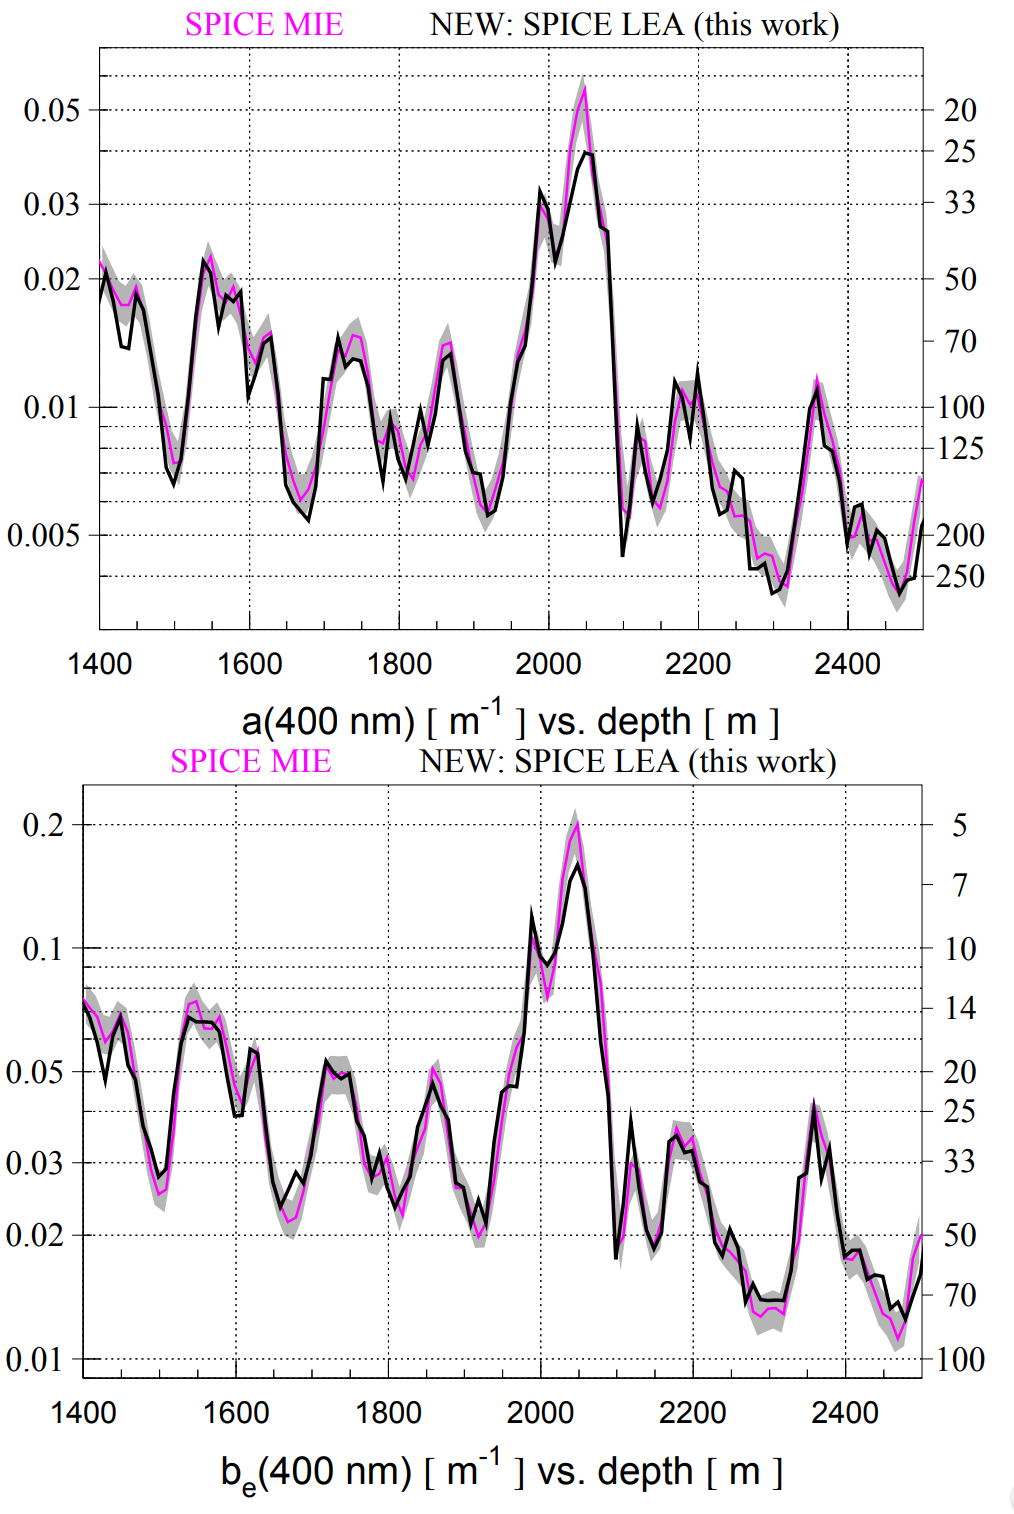
\includegraphics[height=3.5in]{chapter5/img/spiceleacoefficients.png}}
\end{minipage}
\caption{\textit{Left}: Top view of the 2008 detector configuration when DOMs on string 63 were used to flash LEDs in a flasher run. Same colors are used for strings located at a similar distance to the central string. \textit{Right}: values of $b_{e}(400)$ and $a(400)$ vs. depth for two different ice models. The scale and numbers to the right of each plot indicate the corresponding effective  absorption $1/a$ and scattering $1/b_e$ lengths in [m]. Both illustrations from Ref. \cite{1412998}.}
\stepcounter{figure}%
\label{fig:2008config}
\end{figure}

Over the years, multiple different ice models have been constructed. For this analysis the SPICELea\footnote{SPICE stands for South Pole Ice. Lea is an addition to distinguish the different model types, but has (as far as the author knows) no special meaning.} model has been set as nominal. This is the most recent model that has significant Monte Carlo background simulations available. It includes an angular sensitivity estimation due to the \textit{hole ice}, a column of ice approcimately 30 cm in radius immediately surrounding the strings with an increased amount of scattering. More information about this model can be found in Ref. \cite{1412998}.
\subsection{Systematic uncertainties}
The characteristics of the ice are complex. Dust particles, the tilt in the ice sheets, etc. result into non-negligible uncertainties in the ice model. Data from the flasher runs are compared to simulation and this verification was used to quantify the uncertainty on the measured values of $b_e(400)$ and $a(400)$. From this, it was determined that $(+10\%,0), (0,+10\%)$ and $(-7.1\%,-7.1\%)$ uncertainties on the scattering and absorption coefficients, respectively, was a conservative estimation.

\section{IceCube event topology}
The compressed waveforms are refolded to approximations of the original waveforms using average single-photoelectron pulse shapes as can be seen in Figure \ref{fig:waveform}. The timing, shape and amplitude of the reconstructed waveforms in all the DOMs in an event are used to characterize the event topologies in the detector. Different interactions give rise to several possible signatures in the detector. Energetic muons propagate several hunderds of meters in the ice and give rise to tracks, whereas electrons and hadrons are stopped almost immediately, giving rise to cascades (see Section \ref{sec:propagation}).

\begin{figure}[t]
\centering
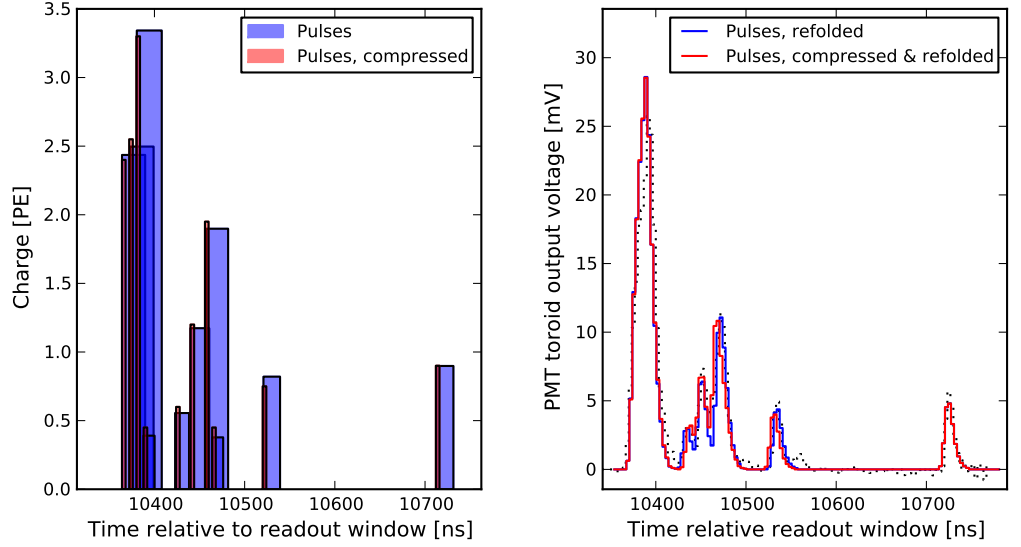
\includegraphics[width=\textwidth]{chapter5/img/waveform.png}
\caption{\textit{Left:} pulse information illustrated with blue bars; the leading-edges time, width, and charge of the pulse are given by the left edge, width, and height of the bar, respectively. The red bars show the same after SuperDST compression. \textit{Right: }Reconstructed pulses using the full pulse profiles in blue are compared to an approximation of the original waveform that is obtained by convolving the pulse times and charges with an average single-photoelectron pulse shape. Figures from Ref. \cite{waveforms}.}
\label{fig:waveform}
\end{figure}

The track-like events, originating from charged-current muon neutrino interactions, provide an angular resolution at a typical angle of 1$^\circ$ for well-contained and reconstructed tracks at 1 TeV and improves to $\sim 0.3^\circ$ for neutrinos with an energy of 1 PeV \cite{Aartsen:2018ywr}. Cascades, originating from electromagnetic or hadronic cascades, result in a more spherical light generation in the detector. Well-contained shower events have an average deposited energy resolution of around 15\%. These event types are shown in more detail in Figure \ref{fig:ICinteractions2}.
 

\begin{figure}
\centering
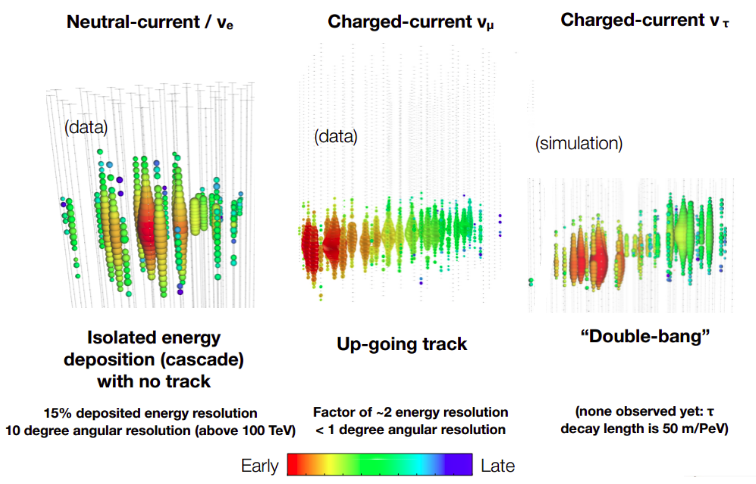
\includegraphics[width=\textwidth]{chapter4/img/ICinteractions2.png}
\caption{Neutrino interactions in the IceCube detector have two distinct types of interactions: cascades and tracks. Energetic taus are theorized to have double-bang signatures but have not undeniably been seen. Colors determine the timing of hits in the optical modules in the ice. Illustrations from the IceCube collaboration \cite{kjeroSignatures}.}
\label{fig:ICinteractions2}
\end{figure}


\section{Future upgrades}
The last couple of years there has been a large focus on improving the physics work that can be done in the IceCube experiment. Several projects are in the pipeline, are under R\&D, and/or have been funded to improve the full analysis case of the detector(s).

Lower-energy neutrinos can be detected with a denser infill with other optical modules (the Upgrade, see Section \ref{subsec:upgrade}), cosmic ray measurements can be improved with a complementary scintillator array to the IceTop tanks \cite{Collaboration:2017tdy} and small air cherenkov telescopes \cite{Auffenberg:2017vwc}. Also, the detection of ultra-high-energy neutrinos could be made possible with a larger infill of the current IceCube in-ice array (Gen2) or radio antennas. Below a brief summary of projects that could be of potential importance to this analysis is given.

%\subsection{Scintillators}
%During the Antarctic summer of the 2017/2018 season, several scintillator prototypes were installed as proof-of-concept for a full scintillator\footnote{Scintillators collect light that is produced by particles travelling through matter that is excited by the relativistic particle (Bethe-Bloch formula).} array with a similar coverage of the current IceTop array. One station would consist of 7 scintillator panels; one as the center and the remaining six in a hexagonal shape around the center. A total of 37 stations result in 259 panels in total with an instrumented area of $\sim 388$ m$^2$ \cite{Collaboration:2017tdy}. This main purpose of this setup is twofold:
%\\
%\begin{itemize}
%\item \textbf{Measure the attenuation due to snow.} IceTop tanks suffer from snow accumulation and many IceTop analyses have this effect as their main systematic error. Electromagnetic components of air showers have short attenuation lengths in snow, resulting in a clear difference of signal rates for tanks that accumulated more snow than others in the course of the years since deployment. The uncertainty in the attenuation function, that depends on the distance to the shower axis, muon number, snow depth, energy, and zenith angle is expected to increase the estimated 6\% systematic uncertainty on the energy spectrum in the following years. A reference signal from the scintillators can reduce this systematic uncertainty.
%\item \textbf{Improve low-energy detection efficiency.} Scintillators are able to efficiently detect air showers to lower energies than currently possible with IceTop detectors only.
%\item \textbf{Signal determination.} The setup could also be used in a similar fashion as the Pierre Auger upgrade was used to distinguish the muon and electromagnetic contributions \cite{Aab:2016vlz}. 
%\end{itemize}
 
%\subsection{IceAct}
%The main backgrounds in most IceCube analysis (including the one described in this work) are from atmospheric muons and muon neutrinos. IceTop has been shown to act as a veto for these events and is used in some analyses \cite{Tosi:2017zho}. A possible complementary extension of the IceTop detector is based on small Air Cherenkov Telescopes (ACTs), called IceACT \cite{Auffenberg:2017vwc}. ACTs use air as the active volume for light production and use cameras to detect light produced by cosmic rays. Downgoing atmospheric neutrinos could be vetoed as they are also accompanied by air showers on the surface. Currently, several prototype setups are deployed and tested on South Pole. One prototype telescope consists of 61 pixel SiPM camera with a 60 mm focal plane radius as the central part. One station would consist of a central telescope with six others surrounding it in a hexagonal shape. Each telescope would be oriented to a different point in the sky, optimizing the total field of view. An array covering the IceTop and IceCube detectors is proposed but still being discussed. Stations further away could also be included to further optimize the veto capabilities and would include fewer than 7 telescopes as the detection of a very inclined cosmic ray with one telescope shields more modules deep in the ice than vertical cosmic ray events.

\subsection{IceCube Upgrade}
\label{subsec:upgrade}
\begin{figure}[t]
\centering
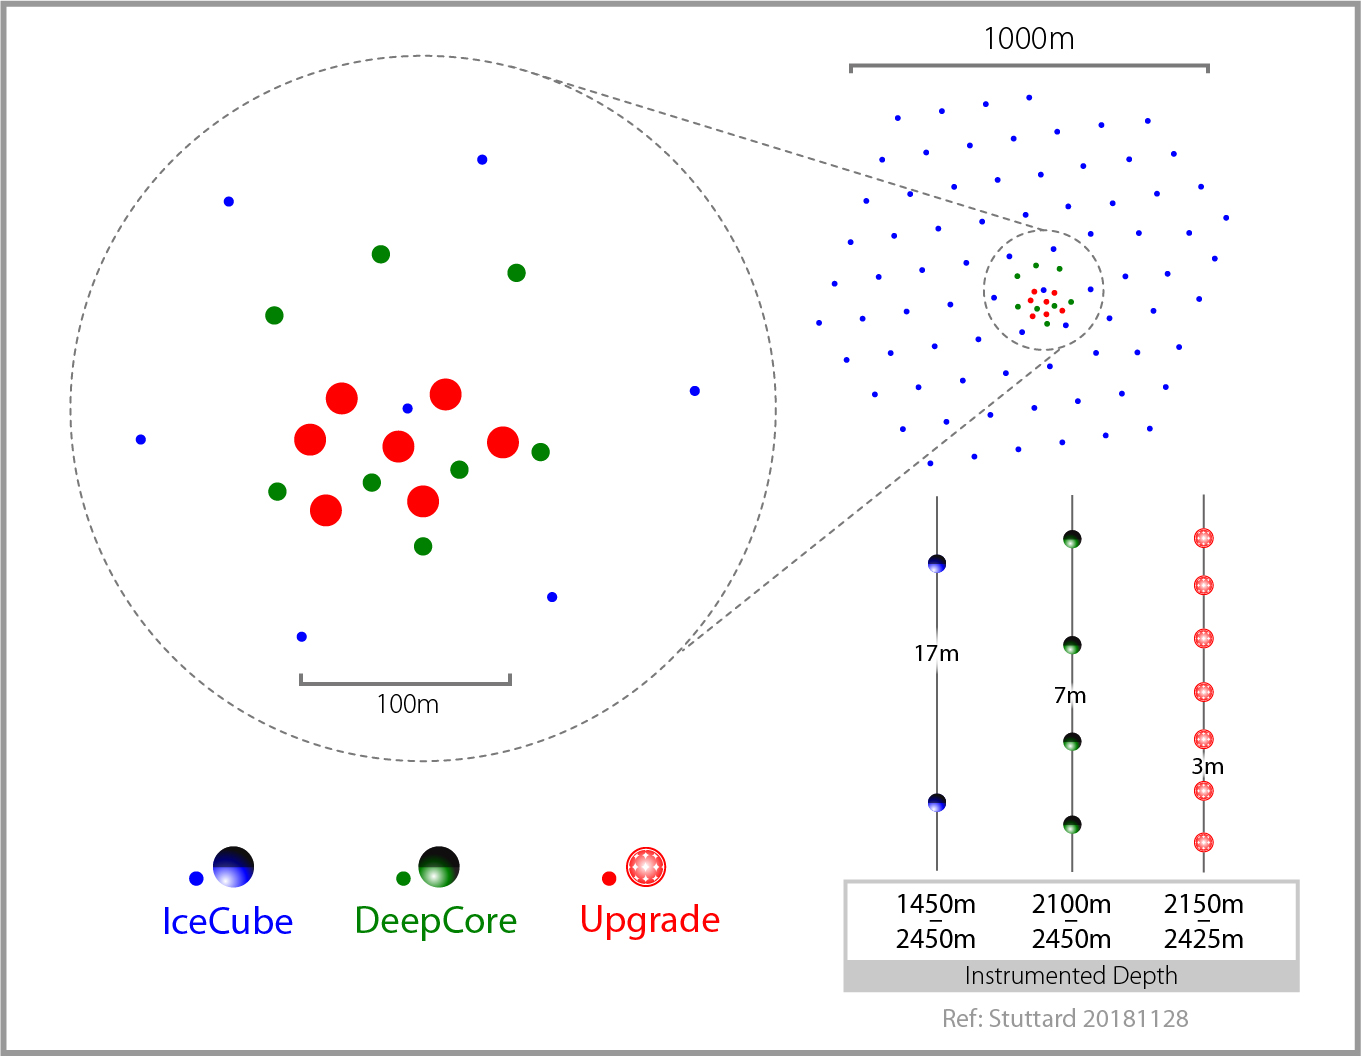
\includegraphics[width=0.8\textwidth]{chapter5/img/ICUpgradeLayout_V3.jpg}
\caption{Top view of the Upgrade infill (red circles) within the DeepCore array (green) and the whole IceCube detector (blue). The area of the circles is representative of the instrumented photocathode density on a given string. Illustration from the IceCube collaboration.}
\label{fig:upgrade}
\end{figure}

In 2018, a funding proposal for a dense 7-string infill of DeepCore was accepted by the NSF and was effective from the beginning of October later that year. This infill would have DOMs separated 2.4 m apart and start from a depth of 2140 m, reaching to 2440 m deep in the ice along seven new strings (see Figure \ref{fig:upgrade}). This very dense array would allow low-energy and oscillation experiments to reach much better sensitivities. Also, very dim tracks such as the ones from particles with an anomalous charge lower than $e$, might be easier to distinguish from low-energy muons that produce more Cherenkov light. 

Because this project involves a restart of the drill, it also serves as a testbed for new optical modules. The Upgrade is the first step towards the much bigger Gen2 project. New types of optical modules would be used with higher angular acceptances than the currently used DOMs that have one large downward facing PMT. Examples are D-Eggs, which have two PMTs at each end of an ellipsoid glass \cite{Ishihara:2017vxn}, and mDOMs, where multiple smaller PMTs are positioned in a ball-shaped optical module \cite{Classen:2017sng}. 

A camera system could also be included in the new optical module designs and should help to improve the properties of the ice after refreezing \cite{Collaboration:2017chl}. Another camera system, the Precision Optical Calibration Module (POCAM) should further improve our understanding of the ice characteristics and accurately determine the efficiency and angular acceptance of the IceCube DOMs \cite{Resconi:2017mad}.\\
\newline
Deployment is currently planned for the 2022/2023 season.

\subsection{IceCube Gen2}
\begin{figure}[ht]
\centering
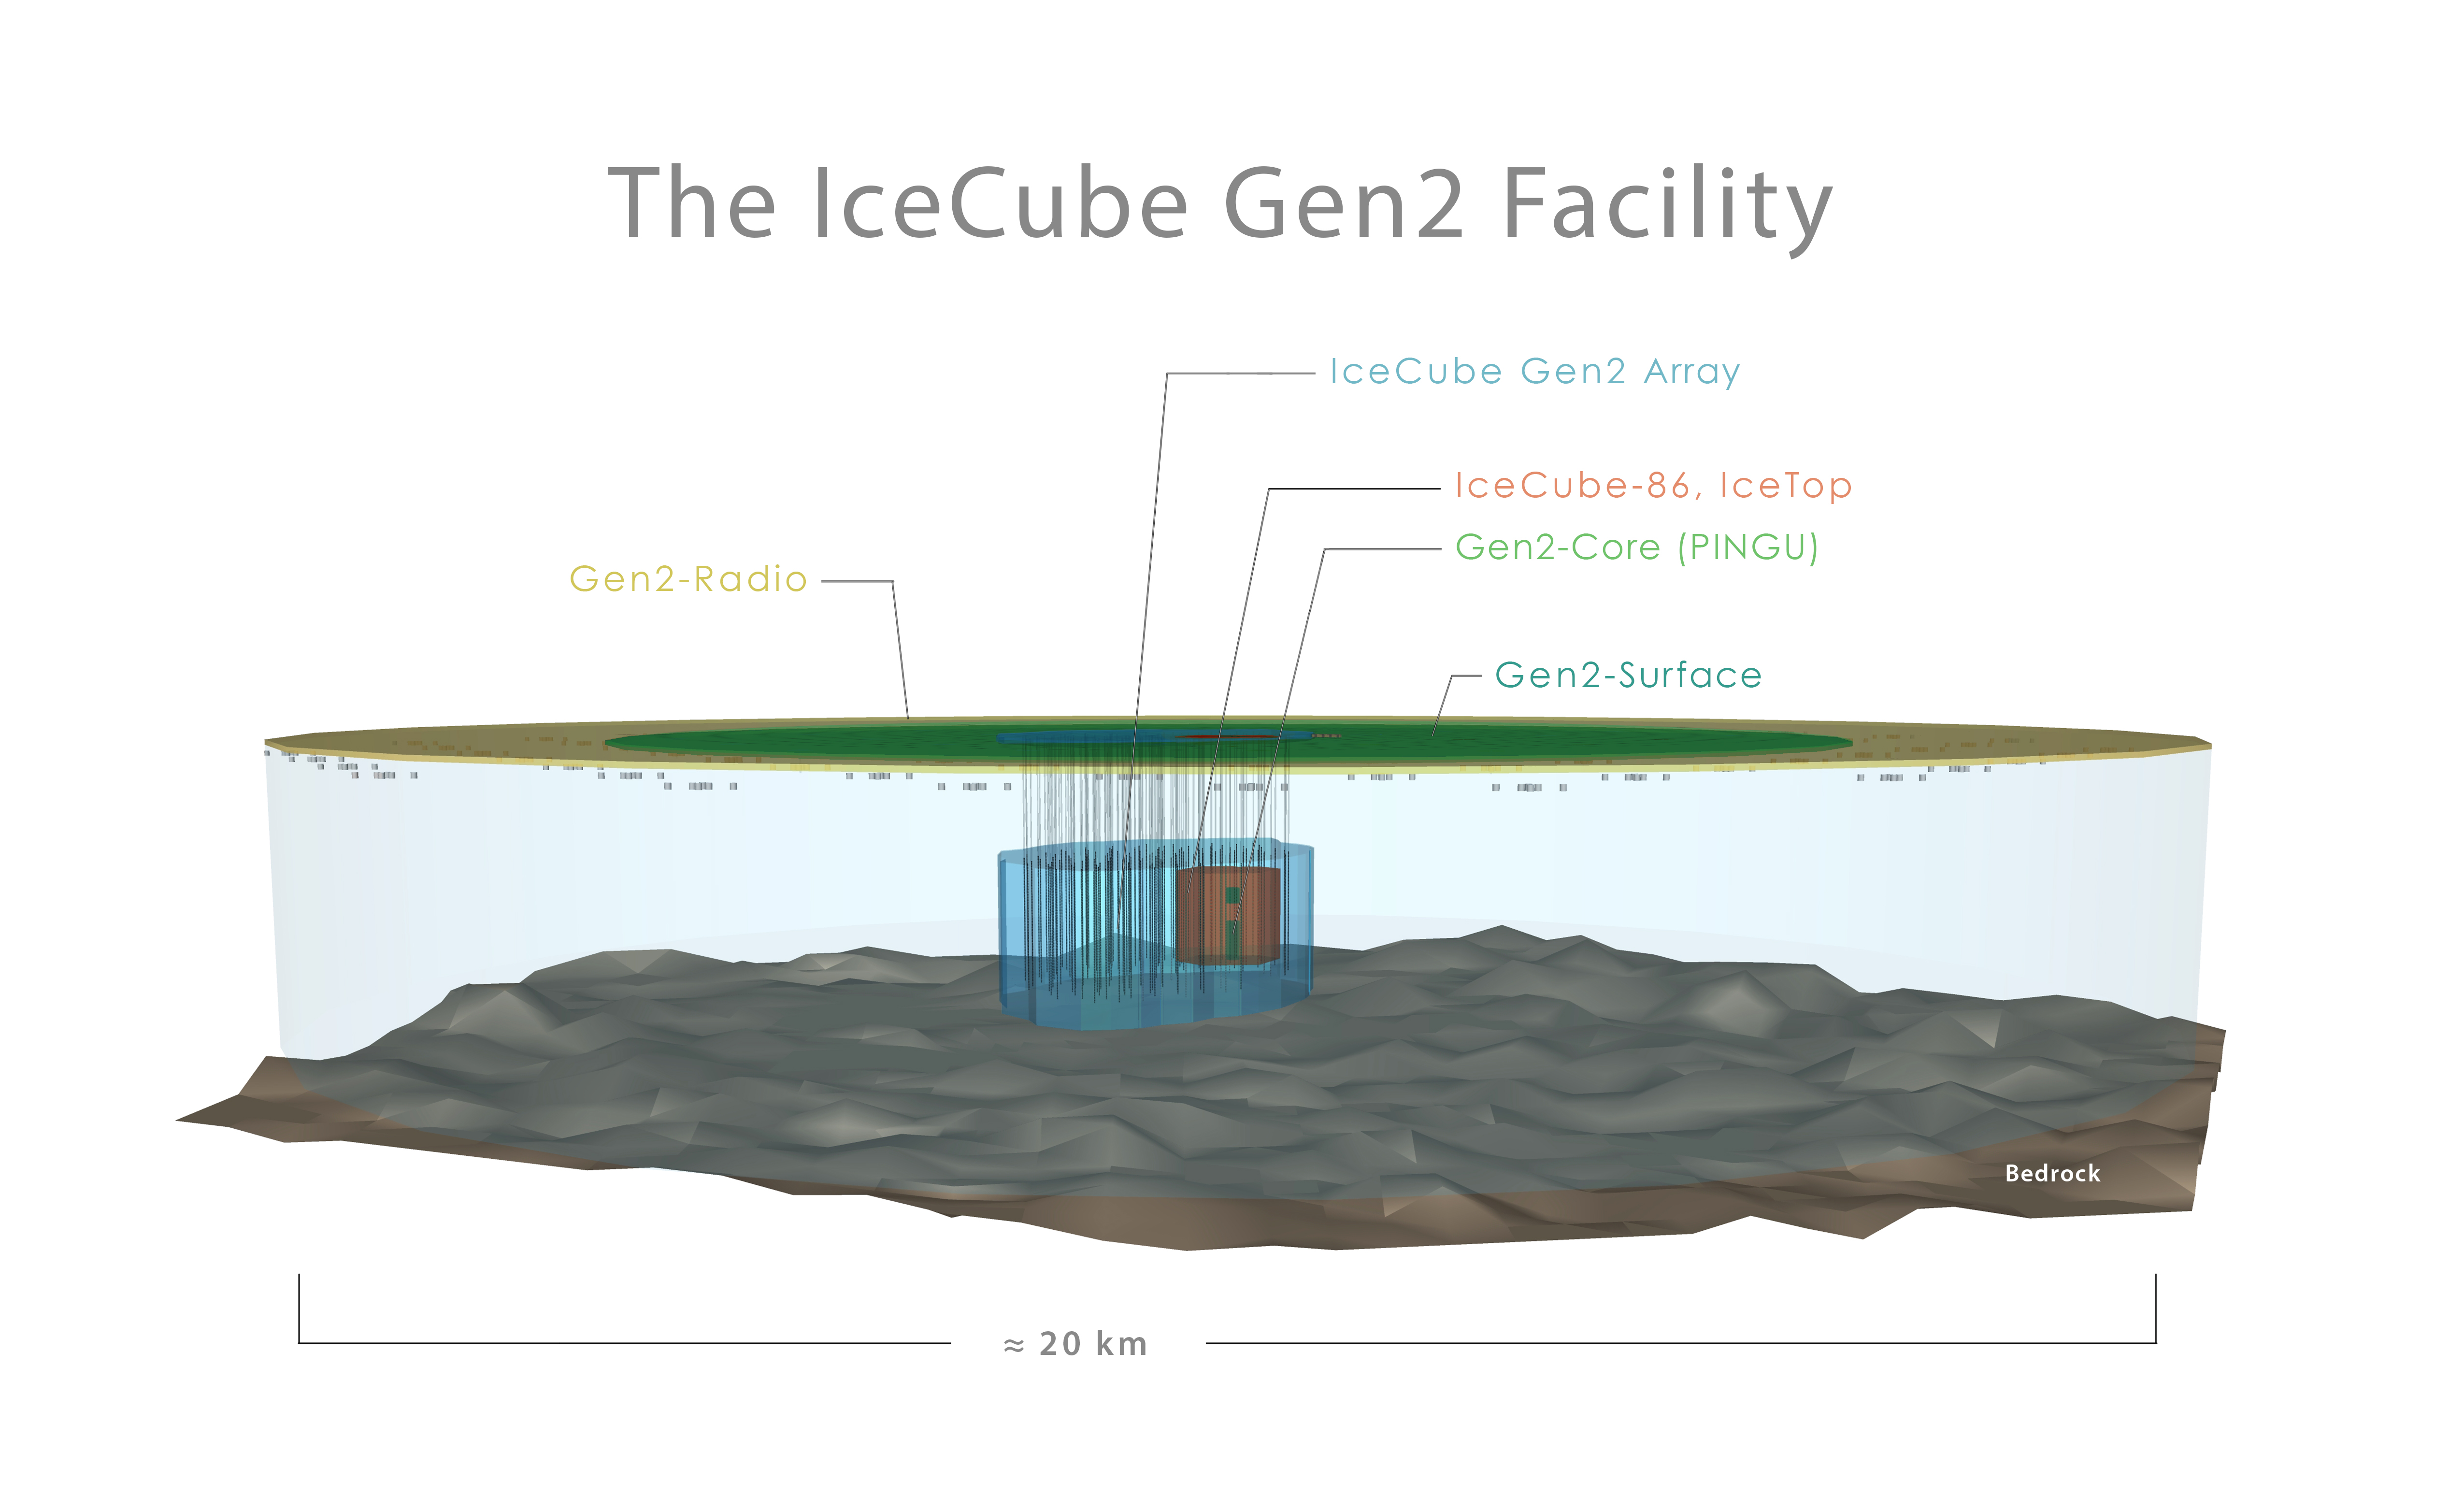
\includegraphics[width=\textwidth]{chapter5/img/gen2_structure.jpg}
\caption{Impression of the possible Gen2 layout. The current IceCube in-ice and IceTop arrays are shown in red/brown. The 10x larger Gen2 in-ice array is given in blue. Possible layouts for the radio array (yellow) and surface array (green) are also listed. From the IceCube collaboration. \textcolor{red}{PINGU zit hier bij, maar nog geen idee of dat er van ga komen of dat het bij de upgrade gaat blijven...}}
\label{fig:gen2}
\end{figure}

\noindent Although the IceCube in-ice array has successfully been able to determine the flux of astrophysical neutrinos and show the detection of a coincident neutrino with a blazar in an active state, a next generation larger detector infill would greatly improve the detection possibilities of astrophysical neutrinos \cite{Blaufuss:2015muc}. A 10 km$^3$ volume of clear glacial ice would allow for a much higher detector acceptance of high-energy neutrino interactions, helping in searches for point sources, beter characterizing the spectral and flavor properties, and search for cosmogenic neutrinos among others. Point sources and cosmogenic neutrinos have, for now, not been observed even though the detector has been running stable for a couple of years. There is also only a small set of unambiguous astrophysical neutrinos. It would take extremely large running operations from the current detector (without hardware failures that are prone to happen more and more) to gather enough events for meaningful statistics. A much larger instrumented volume, such as the one proposed, is predicted to have an increase in sensitivity to transient source densities and rated by about two orders of magnitude \cite{Ahlers:2014ioa}. Also, a large extension of the active volume could help to look for long tracks originating from SMPs. Although much is undecided, the plans are to have an extra surface array for cosmic ray detecton and a radio array for the highest energy neutrinos along the in-ice array.\\
\newline
\textcolor{red}{Deployment is planned for ???}

\subsubsection{In-ice infill}
The current design for the Gen2 string configuration would be $\sim$120 cables with an inter-string spacing around 250 m to 300 m. This much coarser spread of strings will result in a loss of sensitivity for neutrino events of the order of couple of TeV but would not affect the measurements of the very energetic astrophysical neutrinos. Measurements of the absorption lengths in function of the depth in the ice indicate that the instrumentation of the strings could be extended with an additional 250 m in total. This total depth is comparable to the current depth of the IceCube detector, meaning the surface area should reach to an exposed area of $\sim$ 10 km$^2$. This would result in a drastic sensitivity improvement of (near-)horizontal muons traversing the ice that are too energetic to be contained in the current detector.
\subsubsection{Surface array}
The size of the IceTop array is too limited for most analyses to be used as a veto for most analyses. Therefore, the prospects of a surface array for the Gen2 extension would have much larger designs \cite{Euler:2015oen}. The geometry and optimal type of detector that should be used for this configuration is still under design.
\subsubsection{Radio array}
\label{subsub:radio}
To achieve an improved sensitivity to neutrinos in the $10^{16} - 10^{20}$ eV energy range, including GZK neutrinos, an additional radio-pulse neutrino detector could be constructed. At the critical energy of around 100 PeV, the origins of cosmic rays transitions from the highest-energy galactic sources to the even more extragalactic cosmic rays. A good review of radio emission from cosmic rays is given in Ref. \cite{Schroder:2016hrv}. There are ongoing experiments that act as a proof-of-principle for the radio technique in the ice: ARA (Askaryan Radio Array) \cite{Allison:2015eky}, close to the IceCube detector at South Pole (see Figure \ref{fig:aerialview}) and ARIANNA (Antarctic Ross Ice Shelf Antenna Neutrino Array) \cite{Glaser:2018ifj} on the Ross Ice Shelf at the antarctic coast.



\iffalse
\section{Search strategies}
%heel veel hiervan: \url{https://arxiv.org/pdf/1806.05696.pdf}
The IceCube experiment consists of about 300 people from 50 institutions spread over 12 countries. A wide variety of senior scientists, graduate students, technicians, software specialists and engineers works on the continuous running operations to keep the detector running in both hardware and software. Most other people focus on physics analyses that range from low-energy oscillation physics to the rare highest-energy neutrino interactions in the ice. Below I give a general and very brief overview of the IceCube analyses. Other examples, which are not mentioned below, are neutrino cross section measurements \cite{Aartsen:2017kpd}, inelasticity measurements \cite{Aartsen:2018vez}, studies in hadronic interactions from cosmic ray interactions \textcolor{red}{SAMDRCITEREN}, and sterile neutrino searches \cite{TheIceCube:2016oqi}.

\subsection{Multimessenger astronomy and astrophysical neutrinos}
\label{subsec:multimessenger}
\begin{figure}[t]
\centering
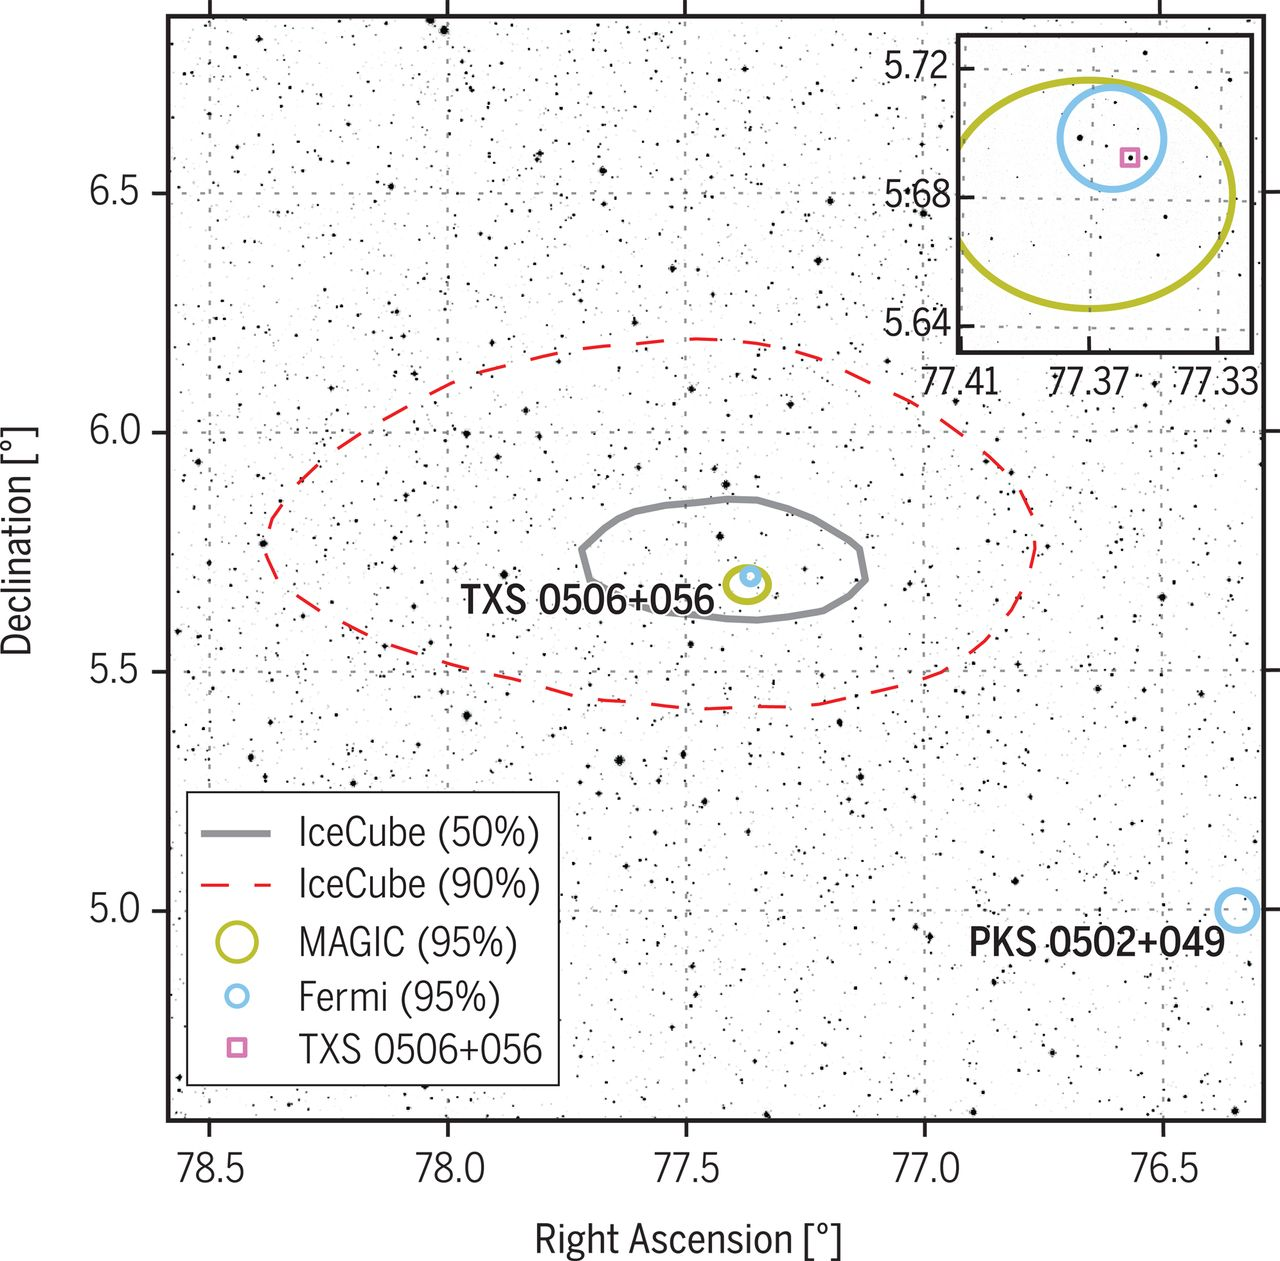
\includegraphics[width=0.4\textwidth]{chapter5/img/blazar.jpg}
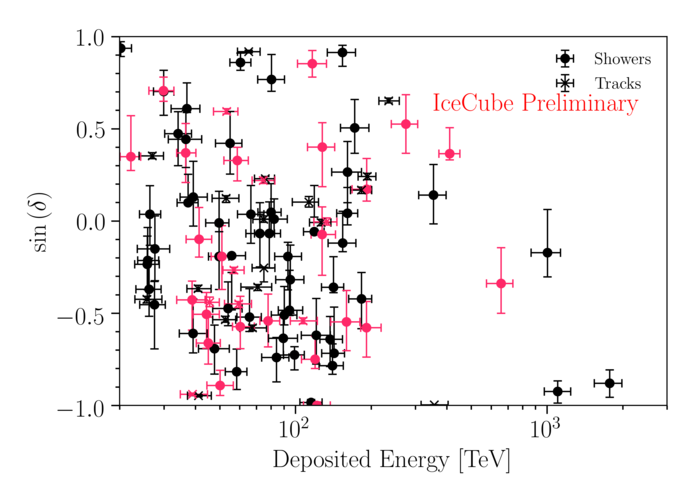
\includegraphics[width=0.57\textwidth]{chapter5/img/highenergyevents.png}
\caption{\textit{Left:} Sky map around the presumable blazar source with the gamma-ray sources detected by Fermi and MAGIC overlain. These are in excellent agreement with the IceCube neutrino containment region. \textit{Right:} Map of showers (cascades) and tracks with their respective declination and deposited energy in the detector.}
\label{fig:blazarandastro}
\end{figure}

The globally coordinated effort in joint searches and observations of cosmic rays, neutrinos, gravitational waves, and electromagnetic radiation is called \textit{multimessenger astronomy}. As an example: a single source, such as a blazar, is expected to produce several signatures that would individually be prone to large uncertainties or even a lack of detection from background events. The IceCube collaboration has a good track record of detecting astrophysical neutrinos and measuring the diffuse flux \cite{Klein:2018fnn,Aartsen:2017mau}. Individual sources long remained unidentified until the joint effort of multiple collaborations such as IceCube, Fermi-LAT, MAGIC, AGILE, and others\footnote{A full list of participating collaborations can be found here \cite{IceCube:2018dnn}.} observed a coincidence with a high-energy neutrino from IceCube and a flaring blazar \cite{IceCube:2018dnn}. The detection of the neutrino, referred to as IceCube-170922A, triggered an extensive multiwavelength search over the electromagntic spectrum ranging from radio frequencies to $\gamma$-rays. Spatial and temporal coincidence of the estimated 290 TeV neutrino with a $\gamma$-ray emitting blazar suggest that high-energy neutrinos have blazars as possible origins. Results of the combined analysis for the blazar called TXS 0506+056 is shown in Figure \ref{fig:blazarandastro}. 

\begin{figure}[t]
\centering
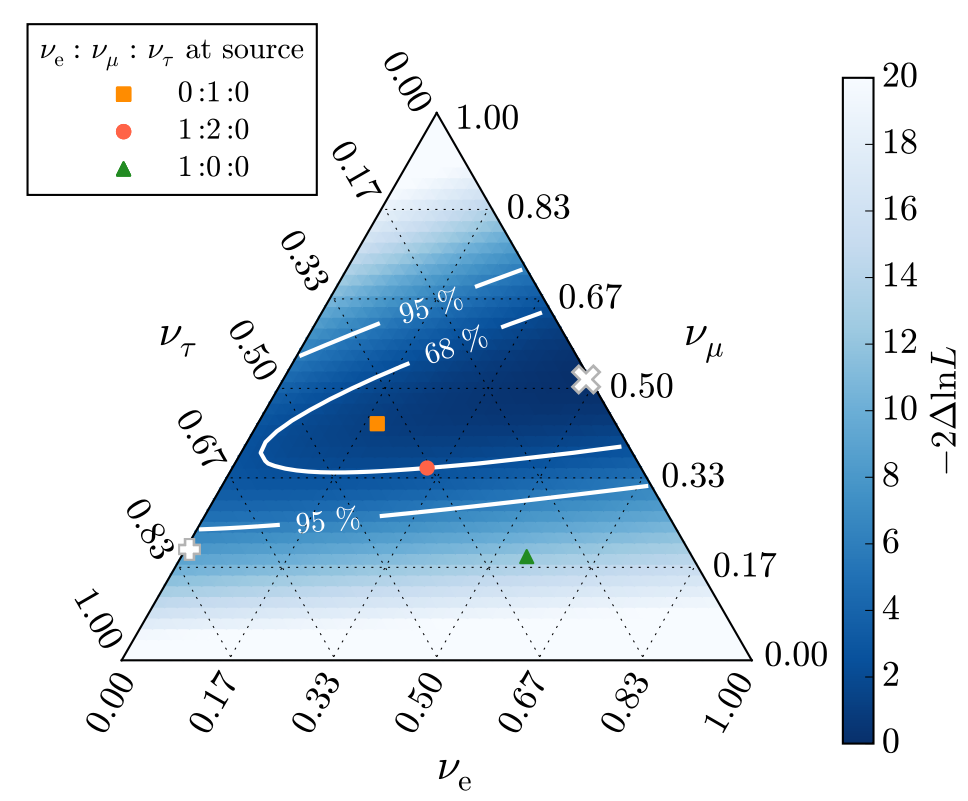
\includegraphics[width=0.6\textwidth]{chapter5/img/FlavorTriangle.png}
\caption{Scan of the flavor composition measured at Earth. The axes show the relative abundances of $\nu_e, \nu_\mu$ and $\nu_\tau$. The best fit is marked with an ``x'' and compared to three possible scenarios of neutrino abundances at the source. Propagation of neutrinos show different measurements at Earth due to oscillation effects. From Ref \cite{Aartsen:2015knd}.}
\label{fig:triangle}
\end{figure}

\subsection{Oscillations}
\begin{figure}[t]
\centering
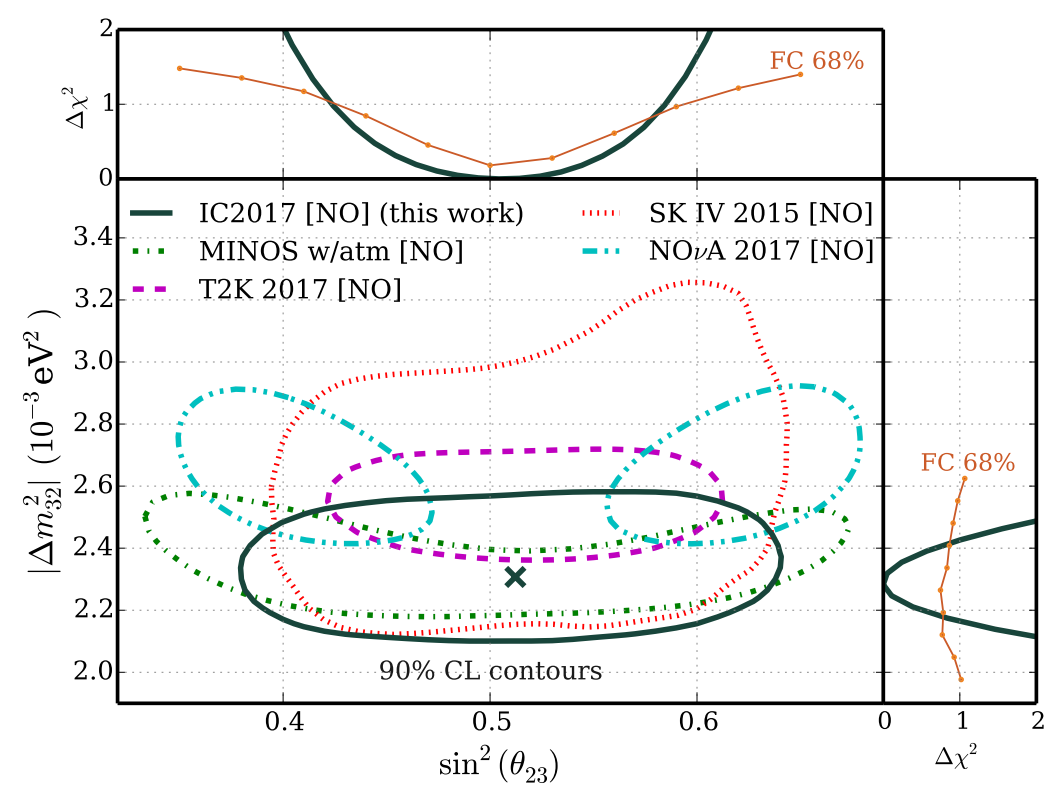
\includegraphics[width=0.7\textwidth]{chapter5/img/oscillations.png}
\caption{Comparison of the $\sin^2 \theta_{23}$ and $\left| \Delta m^2_{32}\right|$ measurements between IceCube, Super-K, T2K, MINOS and NO$\nu$A. Normal mass ordering is assumed. Figures from Ref. \cite{Aartsen:2017nmd}.}
\label{fig:oscillations}
\end{figure}

As discussed in Section \ref{subsec:particlemixing}, neutrinos oscillate in between flavor due to their mixing of mass and interaction eigenstates. Atmospheric neutrino ``beams'' that reach IceCube are ideal candidates to study this behavior at higher energies than most reactor- or accelerator-based experiments. As these particles arrive from all directions, they travel around 10 km (down-going) up to 12,700 km (up-going) before reaching the detector. As this path length is related to the measured zenith angle, a study that combines the measured energy with the angle is able to measure $\sin^2 \theta_{23}$ and $\left| \Delta m^2_{32}\right|$ comparable to world-leading experiments as shown in Figure \ref{fig:oscillations}. 

\subsection{Galactic supernovae}
A supernova explosion close by would result in a general rise of the noise rate of the detector (see Sections \ref{subsec:triggers} and \ref{subsubsec:supernovae}). The IceCube detector should, in theory be, sensitive to supernovae explosions not too far in our galaxy \cite{Baum:2017rty} and is a member of the Supernova Early Warning System (SNEWS) \cite{Kowarik:2009qr}.
\fi

\section{Beyond the Standard Model searches}
The IceCube experiment consists of about 300 people from 50 institutions spread over 12 countries. A wide variety of senior scientists, graduate students, technicians, software specialists and engineers works on the continuous running operations to keep the detector running in both hardware and software. Most other people focus on physics analyses that range from low-energy oscillation physics to the rare highest-energy neutrino interactions in the ice. Below I give a general and very brief overview of some IceCube analyses that search for beyond-the-Standard-Model physics.

\subsection{Lorentz invariance violation}
\begin{figure}[t]
\centering
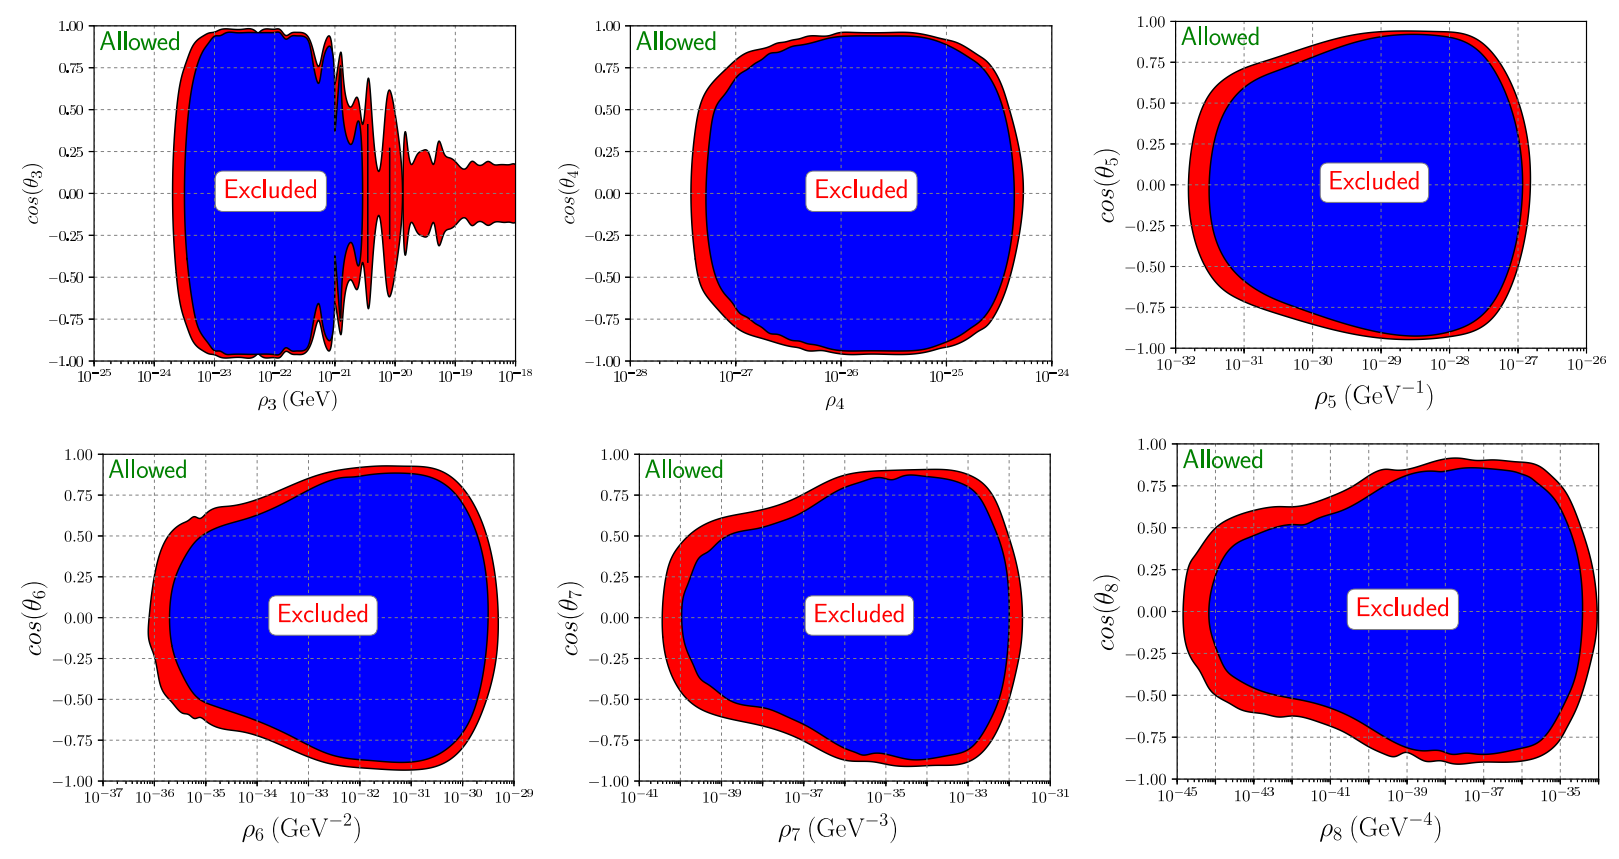
\includegraphics[width=0.95\textwidth]{chapter5/img/LV.png}
\caption{Regions excluded at 90\% (99\%) C.L. in the LIV parameter space in red (blue). $\rho$ is related to the strength of the LIV and $\cos \left(\theta_d\right)$ is a combination of coefficients defining LIV in the effective Hamiltonian of Standard Model Extension \cite{Colladay:1998fq}. The subscript $d$ refers to the power of the corresponding operator in the Hamiltonian. More information in Ref. \cite{Aartsen:2017ibm}.}
\label{fig:lv}
\end{figure}

\textcolor{red}{is dit  nu goed uitgelegd of niet?\\}
Lorentz symmetry is one of the foundations of the SM: fundamental laws in nature are thought to be independent of the observer's inertial frame. Some SM extensions allow for spontaneous breaking of Lorentz symmetry and can lead to Lorentz-invariance violating (LIV) effects. Examples are string theory or quantum gravity. Some effects that would follow from these extensions are incorporated in the Standard Model Extension (SME) \cite{Colladay:1998fq} and although the size of LIV effects should be suppressed by the Planck scale ($\approx 10^{19}$ GeV). They could manifest themselves in, e.g., oscillations of atmospheric neutrinos that would modify the observed energy and zenith angle distributions of atmospheric muon neutrinos observed by the IceCube experiment. The LIV effects are often parametrised by two paramameters: $\rho_d$ and $\cos \left(\theta_d\right)$ (which are explained in the capture of Figure \ref{fig:lv}), where $d$ refers to the power of the operator in the Hamiltonian. The energy reach of the IceCube detector makes it possible to go to dimensions up to 8 whereas most other experiments are sensitive up to dimension $d=3$ or $d=4$. This analysis was done first in the 40-string configuration \cite{Abbasi:2010kx} and later redone with the full detector configuration \cite{Aartsen:2017ibm}. Results for $3 \leq d \leq 8$ are shown in Figure \ref{fig:lv}.

\subsection{Dark matter}
\label{subsubsec:DM}

\begin{figure}[ht]
\centering
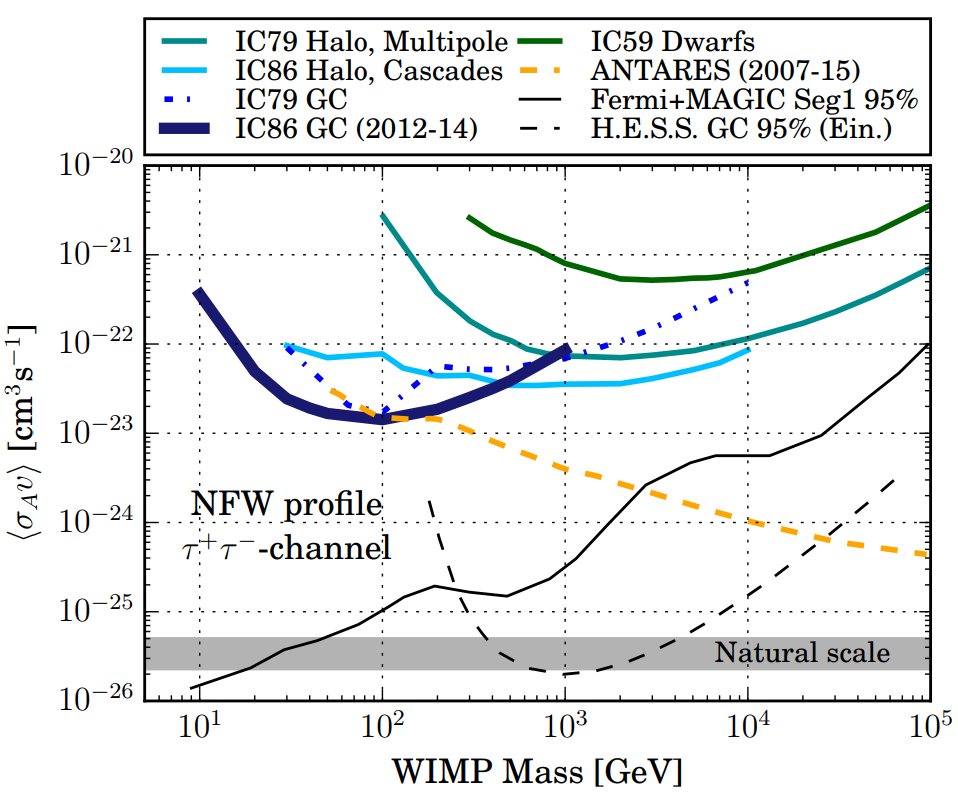
\includegraphics[width=0.65\textwidth]{chapter5/img/dm.png}
\caption{Upper limits of $\langle \sigma_A v\rangle$ in function of the WIMP mass from different experiments.}
\label{fig:dm}
\end{figure}

The large amount of evidence to support the existence of dark matter (DM) was given in Section \ref{needforBSM}. Many ongoing experimental efforts try to search for these elusive particles\footnote{Assuming that they are in fact particles.}. Collider experiments try to produce these particles by SM interactions (\textit{production searches}), other experiments try to measure their interaction with SM particles through nuclear recoil (\textit{direct detection}). It should also be possible to search for the SM products that are produced when annihilation of DM occurs and the corresponding daughter particles find their way to Earth (\textit{direct detection}). Most searches focus on specific regions in the sky that are more prone to produce a measurable signal. As one characteristic of DM is its non-zero mass, they are expected to be gravitationally trapped in the halo of galaxies or to accumulate in heavy celestial objects nearby such as the Sun or the Earth itself. Since most SM particles never reach us, neutrinos are the only possible messengers. Figure \ref{fig:dm} shows a comparison of upper limits on $\langle \sigma_A v\rangle$ versus WIMP mass\footnote{WIMP stands for Weakly Interacting Massive Particle and is one possible candidate for dark matter.}, for the annihilation channel $\chi \chi \rightarrow \tau^+ \tau^-$ producing tau neutrinos. $\langle \sigma_A v\rangle$ is the WIMP-WIMP annihilation cross section and determines the strength of the expected neutrino flux. The analysis mentioned in the figure searched for signals from the center of the Milky Way \cite{Aartsen:2017ulx}. Other IceCube analyses have searched for dark matter in the Sun \cite{Aartsen:2016zhm,Abbasi:2009vg} and in the Earth \cite{Aartsen:2016fep}.

\subsection{Magnetic monopoles}
The quantum theory of magnetic charge started with a paper by P. Dirac \cite{Dirac60} in which he theorized the existence of magnetic monopoles in a similar fashion as he did to succesfully predict the positron. If $q_m$ is the magnetic charge and $q_e$ the electric charge, Dirac found that the following condition should hold

\begin{equation}
q_m q_e = 2\pi n \ \ \ (n \in \mathbb{Z}),
\end{equation}
and could therefore explain why the electric charge is always quantized, i.e. in integer multiples of an elementary charge. The smallest possible magnetic charge  would be\footnote{At the time of writing his paper, Dirac believed the smallest electric charge was from the electron. Since now we know the down quark holds an electric charge equal to $1/3 e$, the minimal magnetic charge would be equal to $3g_D$.} 

\begin{equation}
\label{eq:mopocharge}
g_D = 2\pi/e = e/2\alpha \approx 68.5e,
\end{equation}
with $\alpha = e^2/\pi$ in natural units. Magnetic monopoles appear automatically in certain Grand Unified Theories that would give rise to these particles after spontaneous symmetry breaking of the GUT group, similar to the Higgs mechanism \cite{HOOFT1974276,Polyakov:1974ek}. Masses are typically of the order of $10^{16-17}$ GeV. They are searched for in IceCube analyses in multiple velocity ranges. Monopoles with velocities close to the speed of light in vacuum produce extremely bright tracks due to their high Dirac charge as shown in Eq. \ref{eq:mopocharge}. At lower velocities ($\approx 0.5c$ to $0.76c$) secondary knock-off $\delta$-electrons could have velocities above the Cherenkov threshold and produce light. Luminescence light from excitation of the ice dominates at low relativistic velocities ($\approx 0.1c$ to $0.5c$). For each of these speed ranges, searches for magnetic monopoles at the IceCube experiment are either in progress (luminescence) or have already set the world's best upper limits on the flux of magnetic monopoles over a wide range of velocities \cite{Aartsen:2014awd}.


\section{Discussion}
\textcolor{red}{Nodig om over te gaan van deel 1 naar deel 2? Zou zeggen van wel. Kort.}
















%\subsection{Muon tracks}
%Ook muonen van atmosfeer, in hfdstk 4 enkel over muonen van neutrinos gebabbeld.
%intro intro
%The track-like structure of the signal allows to find a good ``lever arm'' as the deposited charge on the earliest and latest DOMs provide strong constraints on the event's position, time and direction. As a result, directional reconstruction..... Muons can transit the entire detector, making it difficult to reconstruct the energy of the muon and the parent neutrino. Starting muon tracks are challenging, but more useful to infer the initial energy of the neutrino. Highly relativistic muons are stochastic in nature and the energy loss depends on the energy of the particle. Using equation ??? it is possible to have a better energy reconstruction.
%\subsection{Cascades}
%The light output has a slight asymmetry in the direction of motion, making directional reconstructions challenging. However, these interactions are often calorimetric and therefore allow for nearly complete measurements of the energy and result in a good energy resolution.




%Ook hoofdstuk 6 van: \url{https://edoc.hu-berlin.de/bitstream/handle/18452/17668/yanez-garza.pdf?sequence=1&isAllowed=y}

